\documentclass{ou-report}
\citestyle{agu}

% Dit template is gemaakt door P.J. Molijn in het kader van zijn afstuderen aan de OU in 2014.
% Waarvoor hartelijk dank.
% Minieme maar belangrijke wijzigingen zijn aangebracht door E.M. van Doorn
% Het template is versimpeld door Sylvia Stuurman, 2019.
% Het template is van extra aanwijzingen voorzien door Sylvia Stuurman, 2021.


%\hypersetup{
%pdfsubject={Master Thesis <Titel>, <author>},
%pdfkeywords={keyword1, keyword2}
%}

\begin{document}
\pagestyle{plain}
\title{Dit is de titel van mijn afstudeerverslag}
\author{Ik ben de auteur}
%Title of the thesis
%\title[Subtitle]{Title}
%\author{author}
%\affiliation{
%\begin{tabular}{ll}
%Student: & studentnumber \\
%Date:    & DD/MM/YYY \\
%\end{tabular}
%}
%
%%\coverimage{cover/cover.jpg}
%%            ===============
%\makecover[frontboxwidth=4.6in]
\begin{titlepage}

\begin{center}

%% Insert the OU logo at the bottom of the page.
\begin{tikzpicture}[remember picture,overlay]
    \node at (current page.south)[anchor=south,inner sep=0pt]{
        
\includegraphics[scale=0.7]{cover/logo}
    };
\end{tikzpicture}

%% Extra whitespace at the top.
\vspace*{2\bigskipamount}

%% Print the title in specific color.
{\makeatletter
%\titlestyle\color{ou-cyan}\Huge\@title
\titlestyle\color{red}\Huge\@title{}
\makeatother}

%% Print the optional subtitle in black.
{\makeatletter
\ifx\@subtitle\undefined\else
    \bigskip
    \titlefont\titleshape\LARGE\@subtitle{}
\fi
\makeatother}

\bigskip
\bigskip

by
%door

\bigskip
\bigskip

%% Print the name of the author.
{\makeatletter
\titlefont\Large\bfseries\@author{}
\makeatother}

\vfill

in partial fulfillment of the requirements for the degree of
%in overeenstemming met de vereisten voor het verkrijgen van de graad van

\bigskip
\bigskip

{\bfseries Master of Science}

in Software Engineering

\bigskip
\bigskip

at the Open University, faculty of Management, Science and Technology \\
Master Software Engineering
%aan de Open Universiteit Nederland,

to be defended publicly on Day Month DD, YYYY at HH:00 PM.\@
%in het openbaar te verdedigen op dinsdag 9 september om 15:00 uur.

\vfill

\begin{tabular}{lll}
%% Add additional information here, per faculty requirements, e.g
    Student number: & student number \\
    Course code: & IMA0002\\
    Thesis committee:
        & titles and name of the chairman (chairman), & Open University \\
        & titles and name of the supervisor (supervisor), & Open University
\end{tabular}

%% Only include the following lines if confidentiality is applicable.
\bigskip


\bigskip

\end{center}

\end{titlepage} 


%% Use Roman numerals for the page numbers of the title pages and table of
%% contents.
\pagenumbering{roman}
%% Include an optional title page.

\frontmatter 


\let\cleardoublepage\clearpage

% Optional Dedication, Acknowledgement
%\input{dedication}

%\input{acknowledgement}


%Optional: list of figures, list of tables
%\listoffigures

%\listoftables

%% Include an optional summary page.
%\chapter*{Abstract}

This paper presents a study on browser-based port scanning, a technique that allows for the detection of open ports on a target system through the use of a web browser. The research investigates the optimal strategy for browser-based port scanning, the feasibility of using port scanning to identify specific programs running on a user's system, and the uniqueness of browser-based port scanning fingerprints.

The study demonstrates that browser-based port scanning can serve as an effective alternative to traditional port scanning techniques. The results suggest that browser-based port scanning can accurately identify specific programs running on a user's system. This has concerning implications because browser-based port scanning is a client-side, local operation on the user's system, unlike regular port scanning, which might be leveraged to bypass intrusion detection systems, such as a firewall.

Furthermore, the study estimates the uniqueness of browser-based port scanning fingerprints, which has significant implications for user privacy and internet anonymity. The study reveals that browser-based port scanning fingerprints are distinct enough to be employed as a means of tracking users across various websites, highlighting the need for enhanced privacy measures by modern web browsers.  
%\input{Summary/samenvatting}


\pagenumbering{arabic}

\chapter*{Acknowledgements}

If you would like to, you can thank people here
\chapter*{Abstract}

This paper presents a study on browser-based port scanning, a technique that allows for the detection of open ports on a target system through the use of a web browser. The research investigates the optimal strategy for browser-based port scanning, the feasibility of using port scanning to identify specific programs running on a user's system, and the uniqueness of browser-based port scanning fingerprints.

The study demonstrates that browser-based port scanning can serve as an effective alternative to traditional port scanning techniques. The results suggest that browser-based port scanning can accurately identify specific programs running on a user's system. This has concerning implications because browser-based port scanning is a client-side, local operation on the user's system, unlike regular port scanning, which might be leveraged to bypass intrusion detection systems, such as a firewall.

Furthermore, the study estimates the uniqueness of browser-based port scanning fingerprints, which has significant implications for user privacy and internet anonymity. The study reveals that browser-based port scanning fingerprints are distinct enough to be employed as a means of tracking users across various websites, highlighting the need for enhanced privacy measures by modern web browsers.  

\tableofcontents

\mainmatter

\chapter{Introduction}
% You can start your report by copying the introduction from your VAF. The advice is to rewrite the introduction \emph{after} you did write the remainder of the thesis.

% In the introduction, you:

% \begin{itemize}
% 	\item motivate why this research is important. You can bring forward motivation with respect to society, or show that your research is scientifically interesting; preferably both
% 	\item give some background information
% 	\item describe the goal of your research
% 	\item give the reader an overview of the structure of the remainder of your thesis.
% \end{itemize}

% This sentence is only here to show you how to refer to a source~\citep{Dijkstra-1968}.

% \begin{table}[h!tbp]
% \begin{tabular}{l | r | r| c}
% kolom 1 & kolom 2 & kolom 3 & kolom 4 \\
% \hline
% zon & maan & ster & meteoor\\
% gras & graan & groen & grauw\\
% \end{tabular}
% \caption{Example table}
% \label{table-example}
% \end{table}

% Table~\ref{table-example} shows how to include a table. Note that the first column is left-justified, the right column is centered, and the other two columns are right-justified (because of the \texttt{\{l | r | r | c\}}). More information: \url{https://en.wikibooks.org/wiki/LaTeX/Tables}. 

% \texttt{[h!tb]} means: preferably place the table \emph{h}ere, and if that is not possible, at the \emph{t}op of the page, at the \emph{b}ottom, or on a separate \emph{page}. The same positioning advice can be used in figures. Figure~\ref{fig-example} is an example.

% \begin{figure}[h!tbp]
% 
\includegraphics[scale=0.5]{LaTeX.png}
% \caption{LaTeX}
% \label{fig-example}
% \end{figure}

% The following chapters are an example of how you could structure your thesis. Do not hesitate to use a different structure!

As the world becomes more digitized, online privacy and user tracking have become major concerns. Websites are collecting vast amounts of data about their visitors, including sensitive information about their devices and browsing behavior. Websites often collect user data, such as search queries, IP addresses, and click behavior, through tracking technologies like cookies and web beacons. The collection of this data can be used for various purposes, such as targeted advertising, personalization, and user profiling.
 
Several studies have explored the implications of user tracking and privacy. Acar et al.~\citescientific{acar2014} found that a significant number of websites are capable of tracking users across multiple visits, posing a potential threat to user privacy. In a similar vein, Mayer and \\ Mitchell~\citescientific{mayer2012} have examined the privacy implications of third-party tracking on the web and have proposed measures for policymakers and developers to address these concerns.

Furthermore, the privacy risks associated with personalized advertising have been analyzed by Komanduri et al.~\citescientific{komanduri2011}, who argue that the collection of user data for this purpose can result in significant privacy risks, since users are often unaware of what data is being collected and how it is being used. Similarly, McDonald et al.~\citescientific{mcdonald2009} have investigated the effectiveness of privacy notices and have found that users frequently do not comprehend the information presented in these notices or the implications of data collection and sharing. These studies and others highlight the importance of protecting user privacy in the context of user tracking and data collection on the web.

Seemingly harmless information, such as browsing habits or search queries, can reveal personal details like interests, location, and even sensitive information like health conditions or financial status. This data is often used for targeted advertising, personalized content, and profiling individuals. However, uncontrolled data collection raises ethical concerns, such as lack of transparency and user control over personal information. Moreover, some tracking techniques may be unlawful in certain countries, violating data protection and privacy laws that impose legal obligations on organizations. Dismissing privacy concerns with the argument `it does not matter' is flawed, as it ignores the potential risks and consequences associated with unregulated data collection and use by online entities. Prioritizing user privacy, promoting transparency, and complying with applicable laws are imperative in safeguarding individuals' privacy on the web.

One popular technique used for user tracking and profiling is browser fingerprinting. It involves collecting various information from a user's browser, such as the user agent string, screen resolution, installed fonts, and plugins. This information can be used to create a unique identifier or \emph{fingerprint} of the user's browser, which can then be used to track the user across different websites and browsing sessions. Cookies, along with browser fingerprinting, are commonly utilized for tracking purposes and are a widely used method for monitoring user activities. They are explicitly referenced in the General Data Protection Regulation (GDPR), which is Europe's largest privacy law~\citeregulatory{gdpr}.

A browser tracking technique that has not been extensively researched is port scanning. Port scanning is commonly used as a network security technique that involves scanning a network for open ports to identify potential vulnerabilities. While not commonly used for user tracking, port scanning can potentially reveal information about a user's device, operating system, and running programs. An important distinction to make with cookies, is that port scanning does not require user consent and is therefore a less transparent tracking technique.

In a high-profile case in 2020~\citearticle{forbes_ebay,ebay_port_scans}, popular ecommerce website eBay used port scanning as a security measure to identify remote access tools on users' systems. Many users were infected with malware at the time, and attackers were using compromised computers to make purchases on the website. eBay used port scanning to detect these remote access tools and prevent malicious users from making purchases. However, security and privacy experts were critical of this security implementation, as scanning the local network has implications for both security and privacy.

The focus of this research will be on port scanning via the browser. There are 65,536 ports provided by the TCP/IP protocol for an IP address in the computer. Among them, the range of well known ports is from 0 to 1023, the range of registered ports is from 1024 to 49,151, and the range of dynamic ports is from 49,152 to 65,535~\citescientific{yuan2020}.
This wide range of ports makes it an interesting topic for research, as each port can reveal sensitive information about a system. Browser-based port scanning has the potential to enhance existing browser fingerprinting methods.

% xprobe2\footnote{\url{https://github.com/binarytrails/xprobe2}},

It is important to differentiate between port scanning in general and port scanning through a browser. 
Scanning ports through a browser is less intrusive and more difficult to detect by intrusion detection systems. This is because port scanning through a browser involves making regular network requests, rather than directly sending probes at the protocol level. Furthermore, a website can passively perform port scanning without requiring user privileges to do so.
Many port scanners have been developed, such as Advanced Port Scanner~\citescientific{el2011}, SATAN~\citescientific{arce2008}, Angry IP Scanner~\citescientific{el2011}, and the most popular open source solution, Nmap~\citescientific{orebaugh201}. However, all of these port scanners focus on port scanning at the protocol level, and they are not limited by abstraction layers that exist in a browser environment. JavaScript APIs do not have access to TCP sockets directly, unlike scanning tools such as Nmap. This severely limits the techniques that can be used to detect open ports. Consequently, the methods used for local port scanning from a browser environment are significantly different from those used by regular scanning tools.

Despite the clear distinction between browser-based port scanning and regular scanning tools, there is limited research on the former. The difference is not just technical, but also relates to the target audience for the scans. Regular scanning tools like Nmap are proactive, whereas websites could use port scanning to passively target their visitors. For instance, a website targeting specific users could scan for particular ports that might reveal sensitive information about this type of user.

Port scanning from the browser can have both positive and negative purposes. It can be used as a security measure to identify remote access tools, or used with malicious intent to gather information about users. However, due to its potential impact on online privacy and security, it remains an essential area for research, especially because these port scans can be done without the consent of the users.

The field of browser-based port scanning has received limited attention in the literature, leaving many intriguing questions regarding its potential impact on privacy. This research focuses on the unexplored use of browser-based port scanning as a browser tracking technique and evaluating its potential implications for user privacy. 

The research has three major contributions:
\begin{itemize}
    \item Estimating the most effective and efficient scanning technique: Before we can assess the privacy risks of browser-based port scanning, it is important to find the most effective scanning technique, efficiency is also a crucial consideration, as port scanning is a time-intensive process. Finding the optimal balance between efficiency and efficacy is critical.
    \item What information browser-based port scanning can reveal about a user: Here we dive into the potential privacy risks of browser-based port scanning, and investigate what information can be revealed through browser-based port scanning.
    \item Estimating the uniqueness of browser-based port scanning fingerprints: Lastly, we estimate the entropy of browser-based port scanning. This contributes to existing browser fingerprinting research by estimating the risk to user anonymity on the internet. 
\end{itemize}

\subsubsection{Thesis overview}

This paper is structured as follows. Firstly, the research questions are discussed, with the primary research question being: \emph{What information can websites extract from clients via browser-based port scanning?} 

Following that, the background chapter explains the basics of port scanning and its ethical and legal implications. Chapter 4 describes related work and  provides an overview of existing literature on browser fingerprinting techniques, as well as related port scanning research.

Subsequently, the study investigates the optimal strategy for browser-based port scanning in Chapter 5, considering efficacy and efficiency. Furthermore, Chapter 6 focuses on the feasibility of using port scanning to identify specific programs running on a user's system, analyzing the privacy implications of this approach, and assessing its effectiveness as a means of tracking users. 
Chapter 7 estimates the uniqueness of browser-based port scanning fingerprints.
Lastly, Chapter 8 concludes the research based on the answers to the research questions, as well as discussing future work.

\chapter{Problem analysis}
Sometimes, it is sufficient to explain the problem and the background of the problem in the introduction. In such cases, you do not need a separate chapter about the problem.

At other times, you can show enough about the problem in your related work chapter.

But often, it is worthwhile to analyse the problem in a separate chapter. You could, for instance, describe a simple example, and show how your example raises questions.


\chapter{Research Questions}

While there has been extensive research on browser fingerprinting, research on browser-based port scanning is lagging behind. Scanning for open ports may take user-tracking to a new level, as individual applications can be detected by a website, leading to specific user profiles and thereby several privacy implications. Therefore, this paper aims to explore the subject of browser-based port scanning as a user-tracking technique, with the following main research question:

\begin{quote}
\textbf{What information can websites extract from clients via browser-based port scanning?}
\end{quote}

% Start by copying everything about your research questions from your VAF. Always rewrite this chapter after you have finished your research results. Often, you will find that you did answer slightly different questions than you thought out before.

% In the introduction, you described the overall goal of your research.
% Here, you formulate your research questions, and you explain them.

% Note that your research questions must be formulated in such a way that you will be able to give meaningful answers in the conclusions of your thesis. The results you have produced must contain the answers to these questions.

% In most cases, one main research question with several subquestions works best.


To answer the main research question, the following sub-questions have been formulated:

\begin{enumerate}[RQ1.]

\item \textbf{How to choose the optimal port-scanning technique for a specific victim client in combination with a specific attack goal?}

The aim of this research question is to compare the efficacy and efficiency of different browser-based port scanning techniques, such as the JavaScript Fetch API, WebSocket API, and XHR API, across multiple browsers and operating systems. 

Different JavaScript APIs may have access to distinct error messages or network responses that could be useful during port scanning. Additionally, the WebRTC API may have access to UDP ports, while the WebSocket API does not. Moreover, certain browsers may block specific port scanning types, while others may have varying levels of security or functionality that could impact the scan's success. 

Furthermore, different scanning techniques may be more useful depending on the attack goal, such as scanning for specific ports, versus enumerating the entire port range. A port scanner application should adapt to the victim's client by detecting the OS and browser, and applying the most effective scanning technique.

Therefore, these techniques will be tested on different browsers and operating systems to identify the most effective methods for browser-based port scanning. This research question will provide a significant scientific contribution, since browser-based port scanning techniques have not been explored in-depth before. There is little research available on scanning techniques, and it is therefore unknown what the limitations and potential of browser-based port scanning is. Furthermore, the scans must be efficient to be a realistic attack vector in practice, and finding the balance between efficiency and effectiveness is a crucial aspect to consider. The outcome of this study will serve as a starting point for future research and will also lay the groundwork for RQ2 and RQ3.

\item \textbf{What information can browser-based port scanning reveal about the underlying operating system?}
The objective of this research question is to investigate what information can be obtained about the underlying operating system (OS) through browser-based port scanning. The results of a port scan can reveal which ports are open or closed, and this information can be used to infer certain details about the system. For instance, the open ports may correspond to specific services running on the system, and this information can be used to determine the OS or potentially even specific versions of software that is being used. 

Additionally, the responses to specific port scans may reveal clues about the configuration of the system, such as the firewall rules or security settings that are in place. By analyzing the results of the port scan, this research will identify what type of information can be learned about the underlying operating system through browser-based port scanning. This research question will add to the existing research on browser fingerprinting techniques.

\item \textbf{What information can browser-based port scanning reveal about specific programs running locally on a user's system?} The purpose of this research question is to collect data using the most effective techniques identified from RQ1 to identify applications running locally on a user's system. Certain applications might listen on specific ports, and by scanning for those ports, a website might be able to identify which applications are running on the user's system.

By collecting this data, the research will be able to identify which applications can be detected using browser-based port scanning. Additionally, different application states will be tested to see if port scanning can be used to detect specific application states. For example, a video chat application will open a port to chat with other participants, and this might be detectable through port scanning. The scientific contribution of this research is to explore a more comprehensive user-tracking technique that has the potential to take user-tracking to a new level by identifying running applications and even specific application states.

\item \textbf{How unique are browser-based port scanning fingerprints?}
While previous research has extensively examined the uniqueness of browser fingerprints, the specific context of browser-based port scanning has not been considered within these analyses. This research question seeks to expand upon the existing body of literature by evaluating the uniqueness of browser-based port scanning fingerprints.

Fingerprints, in the context of web browsing, possess the potential to be highly unique, posing a direct threat to user anonymity and privacy on the internet. Consequently, it is crucial to estimate the true level of distinctiveness that browser fingerprints can exhibit, which we argue has not been fully researched to this day, as the inclusion of browser-based port scanning fingerprints has never been included within these assessments, even though there are 65535 ports on an IP address that can be either open or closed.
\end{enumerate}


% \section{Limitations}

% There are some limitations to consider. One of the limitations is the focus solely on desktop devices rather than other devices, such as mobile devices. This is mainly due to time constraints and the complexity involved in studying multiple device types. However, it is important to note that there may be differences in how port scanning behaves on different devices, and future research could explore this further. While the research plans to explore the differences between different operating systems, such as Windows, Linux and macOS, testing on different hardware configurations will be limited.

% Another limitation to consider is that the research does not focus on potential security risks associated with local port scanning. While it is possible that port scanning could be used for malicious purposes, the primary focus of this research is on privacy concerns. Ethics and legality are not a primary focus of this research either. While it is important to consider the ethical and legal implications of any research study, the primary focus of this research is on user privacy and the behavior of browser-based port scanning. Finally, the study does not examine how often browser-based port scanning occurs in practice, as this has already been researched by Kuchal and Li~\cite{kuchhal2021}. 

% The research questions have focused on the information that can be obtained through browser-based port scanning, such as exploring various scanning techniques, identifying fingerprinting possibilities, and detecting running applications. However, the study has not yet validated the research in a real-world setting. Therefore, a potential topic for future research involves conducting a large-scale user study to assess the effectiveness and potential for user-tracking.

% \section{Research method}


% Here, you describe the method that you used to find answers to your questions. 

% In general, it works well when you describe the method you use for each subquestion.  Therefore, you could opt for an alternative structure, by having subsections for each question, with the method described there as well.

% \section{Validation}
% You should not only describe how you find answers to your research questions, but also how you validate your work: how you will (try to) prove that your answers are indeed answers to your questions.

% Again, you can explain that for each subquestion, or here, in a separate section.


\chapter{Related Work}
% You should find out what other researchers have found out about the problem that you will work on. You do that by searching for scientific sources that relate to the problem that you will work on. Often, the chapter in which you wrote your findings is called `Related Work'. Of course, you can choose another title.

% You may conclude this chapter with a subsection in which you show how what you intend to do differs from what has been researched.

% Try to structure this chapter around \emph{subjects} (instead of naming the different authors or articles that you found sequentially). The idea is that you (and your readers) get a clear view on what is known, and what is still unknown with respect to the problem.

% You can, again, start by copying the related work section from your VAF to this chapter. After having done your research (and often during your research) add what you find.


\section{Browser Fingerprinting}
\label{browser-fingerprinting}

Browser fingerprinting is a well-known technique that has garnered significant attention, thanks to Eckersley's pioneering work in bringing the issue to the forefront~\cite{eckersley2010}. Eckersley developed an algorithm capable of identifying a browser fingerprint with an accuracy of 83.6\%, and it could also detect changes in the fingerprint with 99.1\% accuracy. Subsequent studies have focused on exploring various properties that can be utilized for re-identification, including IP address and user-agent~\cite{yen2012}, fingerprinting the HTML5 canvas~\cite{mowery2012}, detection of installed fonts, time zone, and screen resolution~\cite{boda2012}, as well as measuring the timing of the JavaScript engine execution~\cite{mowery2011}~\cite{rokicki2021}, among others.

Nikiforakis et al.~\cite{nikiforakis2013}, Laperdrix et al.~\cite{laperdrix2016} and Gomez et al.~\cite{gomez2018} have further investigated the practical usage of these techniques, showcasing that this is a real threat to user privacy on the internet. Building upon this research, our paper aims to introduce a fingerprinting technique through browser-based port scanning, focusing on an area with limited existing literature.

\section{Fingerprinting running services and the local network}
% Port scanning in general
Aforementioned browser fingerprinting techniques are lacking research when it comes to fingerprinting the local network. Scanning for open ports on the local network can yield promising results, such as revealing running applications on a system.
Port scanning in general is a well-known technique that is widely used due to its utility for network administrators and its potential use by attackers.
% \footnote{\url{https://nmap.org/book/osdetect-methods.html##:~:text=Nmap\%20OS\%20fingerprinting\%20works\%20by,Then\%20Nmap\%20listens\%20for\%20responses}}
Several tools have been developed to scan ports. Nmap~\cite{orebaugh201} is the most popular tool, and the most relevant for this study, because it can fingerprint systems based on port scanning. 

Nmap is a network scanning tool commonly used by network administrators and both ethical and malicious hackers. It comes preinstalled on Kali Linux, a specialized operating system designed for penetration testing. The tool is able to generate a fingerprint of a target system by sending probes to several ports. Nmap uses TCP, UDP and ICMP probes to directly scan for open ports at the protocol level. Various ambiguities in the standard protocol RFC can
then be exploited due to small implementation differences.
Nmap utilizes an extensive fingerprint database to compare the resulting fingerprint with reference fingerprints. See an example reference fingerprint in Figure~\ref{fig:nmap-fingerprint}. 

\begin{figure}[H]
    \begin{verbatim}
    Fingerprint Apple Mac OS X Server 10.2.8 (Jaguar) (Darwin 6.8, PowerPC)
    Class Apple | Mac OS X | 10.2.X | general purpose
    CPE cpe:/o:apple:mac_os_x:10.2.8
    SEQ(SP=FB-111%GCD=1-6%ISR=104-10E%TI=I%II=I%SS=S%TS=1)
    OPS(O1=M5B4NW0NNT11%O2=M5B4NW0NNT11%O3=
    M5B4NW0NNT11%O4=M5B4NW0NNT11%O5=M5B4NW0NNT11%O6=M5B4NNT11)
    WIN(W1=8218%W2=8220%W3=8204%W4=80E8%W5=80F4%W6=807A)
    ECN(R=Y%DF=Y%T=3B-45%TG=40%W=832C%O=M5B4NW0%CC=N%Q=)
    T1(R=Y%DF=Y%T=3B-45%TG=40%S=O%A=S+%F=AS%RD=0%Q=)
    T2(R=N)
    T3(R=Y%DF=Y%T=3B-45%TG=40%W=807A%S=O%A=S+%F=AS%O=M5B4NW0NNT11%RD=0%Q=)
    T4(R=Y%DF=Y%T=3B-45%TG=40%W=0%S=A%A=Z%F=R%O=%RD=0%Q=)
    T5(R=Y%DF=N%T=3B-45%TG=40%W=0%S=Z%A=S+%F=AR%O=%RD=0%Q=)
    T6(R=Y%DF=Y%T=3B-45%TG=40%W=0%S=A%A=Z%F=R%O=%RD=0%Q=)
    T7(R=Y%DF=N%T=3B-45%TG=40%W=0%S=Z%A=S%F=AR%O=%RD=0%Q=)
    U1(DF=N%T=3B-45%TG=40%IPL=38%UN=0%RIPL=G%RID=G%RIPCK=G%RUCK=0%RUD=G)
    IE(DFI=S%T=3B-45%TG=40%CD=S)
    \end{verbatim}
    \caption{Typical Nmap reference fingerprint~\cite{Lyon2009}}
    \label{fig:nmap-fingerprint}
\end{figure}

The example reference fingerprint provides information about an Apple Mac OS X Server 10.2.8 (Jaguar) operating system running on a PowerPC architecture. It includes details about the OS version (10.2.8), the Darwin version (6.8), and the CPE (Common Platform Enumeration) identifier. It also provides information about various scan results, such as open ports (OPS), window size (WIN), ECN (Explicit Congestion Notification) status, and TCP flags (T1-T7). Additionally, it includes details about the IP ID generation (U1) and ICMP error generation (IE) behavior of the system. This technique enables Nmap to detect specific operating systems and versions, including those for embedded systems such as printers running on custom operating systems.

\section{Identifying web automation bots}
As we aim to detect running programs and services on the local network, it is essential to look at existing research on fingerprinting running services. 

Web automation bots such as Selenium~\cite{selenium} are frequently used for large-scale data collection. These bots are susceptible to being detected via fingerprinting techniques, and can be shown different results compared to the original web page. Detecting these bots is a common research topic in browser fingerprinting techniques. Bot detection often involves multiple browser fingerprinting techniques, making it an interesting area of research. 
% Kuchal and Li~\cite{kuchhal2021} show that browser-based port scanning has been used for bot detection in practice. 
Jonker et al.~\cite{jonker2019} reverse engineered a commercial bot detector and discovered several techniques employed in detecting these bots.

\begin{itemize}
    \item Behavior-based web automation bot detection: Multiple event handlers were added to JavaScript events, such as clicks, mouse movements, a device's orientation, motion, keyboard and touch events.
    \item Code injection routines: Frequent communication with the first party server was found. Within this traffic, fingerprinting information was found. This would allow the server to carry out additional server-side bot detection. After identification, bot-specific code can be injected.
    \item DOM properties: Multiple built-in objects and functions were accessed via JavaScript. Additionally, code was found to scan for bot-only properties, such as the \\\verb|document.$cdc_asdjflasutopfhvcZLmcfl_| property --- a property specific to the ChromeDriver.
    This is known by the Chromium team, but currently marked as a \emph{won't fix} issue, stating that if a website owner wants to block automation tools, they respect their decision~\cite{chromedriver_bug}.
    Vlot~\cite{vlot2018} has done extensive research on this, finding several bot-related properties in obfuscated JavaScript files. 
\end{itemize}

Building on top of this research, Krumnow et al.~\cite{krumnow2022} zoomed in on a specific web automation framework, OpenWPM. OpenWPM is a web privacy measurement framework which makes it easy to collect data for privacy studies on a scale of thousands to millions of websites~\cite{openwpm_github}. The research found that OpenWPM was easily detectable and even found OpenWPM detectors in practice. The results indicate that bot detectors are becoming more prevalent, and data obtained through automation frameworks may not be reliable.

% \subsubsection{Website cloaking}
% Cloaking is a technique where different content is presented to different browsers or bots. While it can serve useful purposes such as providing a more accessible version of a website to users with disabilities, it can also be used for unethical practices like hiding negative reviews or for search engine optimization. However, when detected by search engines, this behavior can result in lower rankings and penalties~\cite{cafarella2004}. Furthermore, malicious websites such as phishing sites may use cloaking to avoid detection.



% It is important to distinguish between port scanning in general and port scanning via the browser, because websites may use browser-based scanning to gather information about a user's system without their consent. Although cookie consent is common due to GDPR~\cite{gdpr} regulations, local network search consent is not, and while less common, scanning the local network does occur.

\section{Port scanning via the browser}

Literature on port scanning via the browser is limited. Kuchal and Li~\cite{kuchhal2021} researched how often websites communicate over the local network. They investigated 100k top domains and 145k malware, phishing and abuse websites. The research discovered that hundreds of websites generate requests to the internal network, including websites in the top 10k domains. While not widespread, it is also not trivial. The study found extensive use of WebSockets, in order to bypass the Same-Origin~\cite{w3c_same_origin_policy} policy.

The study identified four primary reasons for local port scanning: fraud detection, bot detection, native application communication, and developer errors. These causes provide insight into the potential of browser-based port scanning and why it is a crucial research topic. Port scanning may be utilized for various purposes, such as fingerprinting for bot and OS detection, preventing remote access tools for fraud detection, and identifying particular application states for native application communication. Native application communication and detecting remote access tools sets browser-based port scanning apart from other fingerprinting methods, because detecting running programs and potentially even specific application states is not possible with regular fingerprinting techniques. Browser-based port scanning may therefore have the ability to take user-tracking to a new level, by profiling users' running programs on their systems. Additionally, port scanning may contribute to existing browser fingerprinting research as it can be used for detecting bots. 

% WEBSOCKET SCANNING: https://incolumitas.com/2021/01/10/browser-based-port-scanning/
% WEBRTC SCANNING: https://medium.com/tenable-techblog/using-webrtc-ice-servers-for-port-scanning-in-chrome-ce17b19dd474

% Web bot detection techniques.

% Website cloaking.

% Fingerprint-detection scanners.

% Port scanning

% \templateinfo{
% You should find out what other researchers have found out about the problem that you will work on. You do that by searching for scientific sources that relate to the problem that you will work on. Often, the section in which you wrote your findings is called `Related Work'. Of course, you can choose another title.

% You may conclude this section with a subsection in which you show how what you intend to do differs from what has been researched.

% Try to structure this section around \emph{subjects} (instead of naming the different authors or articles that you found sequentially). The idea is that you (and your readers) get a clear view on what is known, and what is still unknown with respect to the problem.
% }

\chapter{Results}
You will have at least one chapter describing your results. Often, it is worthwhile to dedicate a chaoter tp each subquestion. At other times, the methods you used cover several subquestions. In such cases, you could add a chapter for each method.

\chapter{Conclusions and Discussion}

In this document, we researched browser-based port scanning and drew the following conclusions based on our findings: 
\\

\textbf{RQ1: How to choose the optimal port-scanning technique for a specific victim client in combination with a specific attack goal?}

We measured significant variations between different operating systems and scanning techniques. The Fetch API emerged as the most effective JavaScript API for conducting browser-based port scanning, and it proved to be highly efficient across various configurations. This can primarily be attributed to the \emph{no-cors} mode, a setting unique to the Fetch API.
A notable contrast was observed between Ubuntu and Windows. Ubuntu tended to time out network requests whenever possible, whereas Windows adhered to the configured socket timeout settings. This characteristic made browser-based port scanning considerably more efficient on Ubuntu.

We estimate that on Windows/Chrome, which is the most popular combination of OS/Browser, it is possible to scan 1,000 ports within one second (2,500+ on Ubuntu). This makes browser-based port scanning a practical real-world attack on virtually any web page. This is especially concerning because the scanning process can continue throughout a user's entire session on the website, which usually lasts much longer than just one second. 
\\

\textbf{RQ2: What information can browser-based port scanning reveal about the underlying operating system?}

We found that operating systems by default do not expose ports that can be revealed through a browser, with the exception of CUPS on Ubuntu. 
Most OS ports fall under the restricted port range and cannot be detected through browser-based port scanning. 
However, when activating certain services on the OS, some of these services are detectable, such as Hyper-V on Windows.
Furthermore, both Windows and Ubuntu host a \texttt{/etc/services} file which contains a mapping between ports and OS services. This mapping can be used as a foundation for a targeted scan to fingerprint the underlying OS.
\\

\textbf{RQ3: What information can browser-based port scanning reveal about specific programs
running locally on a user’s system?}

Fingerprinting specific programs is more effective than fingerprinting the OS. 
We found many programs from different categories that open a distinct port on the local system, which can be revealed through browser-based port scanning. 
We argue that browser-based port scanning can be used to track users by identifying open ports corresponding to specific applications, and is thereby a direct threat to user privacy/anonymity on the internet, especially when combined with known fingerprinting techniques.

When we can successfully identify open ports and the associated programs, it provides a detailed user profile that can be used for a multitude of purposes. 
These can include personalized web pages or more nefarious use cases such as phishing attempts.
Additionally, this information could be exploited to scan for known exploits of specific programs. 
In essence, the knowledge gained from these open ports not only undermines user privacy, but also establishes a foundation for a range of potentially malicious activities.
\\

\textbf{RQ4: How unique are browser-based port scanning fingerprints?}

We estimate that browser-based port scanning results in highly unique fingerprints, even with a very limited scanning time of only one second. We emphasize that if a mapping between the top 1,000 most popular applications and their corresponding identifiable ports is established, then scanning these 1,000 ports is sufficient to create highly unique fingerprints. These fingerprints would possess an entropy that exceeds 50 when combined with established fingerprinting techniques, which is theoretically enough to uniquely identify any user.

It is essential to note that these results are based on our estimates, and a large-scale real-world study would be necessary to validate these claims in a real-world setting. Nonetheless, we believe that our estimates are not implausible, thousands of ports being either open or closed is a significant characteristic that has been omitted from all existing browser fingerprinting studies, and would greatly enhance these fingerprints.


\subsubsection{Browser-based port scanning is a threat to user privacy and security}

The practice of browser-based port scanning poses a significant threat to user privacy. We argue that browser-based port scanning should be banned by web browsers, or at the very least, users should have to explicitly grant permissions for a website to access their local network. 
We contend that any potential benefits, such as the detection of remote access tools for comprised devices as a security measure, are outweighed by the risks to user privacy and security.
Additionally, we think that using browser-based port scanning as a security measure is inherently insufficient, and there are better --- less intrusive --- established alternatives such as multi-factor authentication, which can prevent hijacked devices from making unauthorized requests.

While the potential defensive mechanism of browser-based port scanning is insufficient, the threats are real.
We established the following threats to privacy in this paper:
\begin{itemize}
    \item Identification of specific open ports: Browser-based port scanning can be used to scan specific ports on a system, corresponding to an application natively opening that specific port. This knowledge can be leveraged to target users who are utilizing a particular type of application or service.
    \item Highly unique fingerprints: Browser-based port scanning, combined with existing fingerprinting techniques, can create highly unique fingerprints, effectively eliminating user anonymity on the internet.
\end{itemize}

While not a focus of this paper, the threats to security are also a significant consideration:
\begin{itemize}
    \item Drive-By Pharming~\citescientific{stamm2007}: Drive-by Pharming was an attack in which a malicious web page, when visited, attempted to change a victim's router DNS settings to gain control over their internet traffic and potentially compromise their credentials.
    \item SOHO Pharming~\citetechnical{sohopharming2013}: SOHO Pharming was an attack that compromised over 300,000 consumer-grade SOHO routers, primarily in Europe and Asia since December 2013. Attackers manipulated DNS configurations, redirected DNS requests, and performed Man-in-the-Middle attacks. The attack targeted various router models, exploited vulnerabilities such as authentication bypass and CSRF techniques, and took advantage of consumer unfamiliarity with router configurations and insecure default settings.
\end{itemize}

\subsubsection{Opt-In Solution for Enhanced Privacy and Security}

The only real benefit to accessing the local network would be a website integrating with its native desktop application. 
Granting explicit permission for this access aligns with established practices for various resources accessed by browsers, such as microphones and cameras.
The Brave browser has already implemented this functionality on both their desktop and mobile browser~\citearticle{brave_localhost}. 
We argue that more mainstream browsers such as Chrome, Firefox, Safari and Edge should adopt this change and give users more control over their privacy. 

West and Rigoudy~\citetechnical{rigoudy2023} have worked on a draft specification to prevent unauthorized private network access from the public internet. 
While this specification is still in draft and not on track to be a W3C standard, we think it should be. 
The principle of least privilege is becoming more popular in modern software architecture. 
Software developed (i.e. browsers) for end users should embrace this principle. 
By adopting the principle of least privilege, software can ensure that users are protected by default, rather than exposed to external threats by default, making it clear that the opt-in approach should be the standard for safeguarding user security and privacy.

In the current landscape, users have several options available to protect themselves against browser-based port scanning. 
One approach involves choosing browsers prioritizing user consent, like the Brave browser. 
However, transitioning to a new browser might pose usability challenges despite its emphasis on privacy.
Another strategy revolves around disabling JavaScript, a step effective in enhancing privacy, but detrimental to modern webpage functionality.
A more realistic alternative is a browser extension, such as the open source \emph{LAN Port Scan Forbidder}~\citeartifact{lanportscanforbidder}. 
This extension prevents unauthorized access to local networks. 
Nevertheless, relying on these measures highlights the conflict between privacy and usability and underscores the need for default user privacy in online environments.
Advocating for a shift where user privacy and security are default settings in modern web browsers remains crucial. 
This approach would alleviate the need for users to resort to these measures and promote a more user-centric approach to online privacy.

\clearpage


\section{Future work}

\subsubsection{Real-world validation}

As we have demonstrated that browser-based port scanning can be used to enhance existing fingerprinting methods and create unique fingerprints, a logical follow-up would be to assess its potential for user-tracking in a real world setting.
The ability to identify and track individuals across various online services and platforms has far-reaching consequences, affecting not only personal privacy but also the potential for data abuse and exploitation.

Existing fingerprinting techniques can already identify users up to a certain point. However, as demonstrated in previous chapters, browser-based port scanning can enhance the uniqueness of existing fingerprinting techniques, and can thereby increase the capabilities of user-tracking.
To evaluate the potential of browser-based port scanning in this regard, conducting a large-scale user study becomes necessary. Such a study would gauge the effectiveness of user-tracking capabilities in a real world setting, when browser-based port scanning is incorporated with existing fingerprinting techniques.

\subsubsection{Scanning private networks}

In our research, we primarily concentrated on using browser-based port scanning to scan the localhost IP address. This focus was chosen because browser-based port scanning is a time-intensive process, and the localhost IP address will generally be the most interesting IP address to scan. However, it is important to note that browser-based port scanning can be extended to scan other private IP addresses, which may reveal sensitive information.

\subsubsection{Browser-based port scanning on mobile}

Preliminary research was conducted on using browser-based port scanning to scan mobile devices. The initial findings did not yield any significant discoveries, but there exists potential for further exploration in this area, as the preliminary research was surface-level and did not dive deep into the network layer.
Mobile devices have become a primary means of accessing online services and platforms for a significant portion of the population. Understanding how browser-based port scanning behaves on mobile platforms is important, as it may have unique implications and challenges compared to desktop environments.

\subsubsection{Unsafe ports}
As mentioned in our research, unsafe or restricted ports refer to a range of ports that are blocked by the browser.
No information can be obtained from these ports, and this is a big limitation of browser-based port scanning. 
Critical ports hosting OS services such as FTP, SSH, and SMTP are protected by this rule, and we cannot obtain information about them.
However, as described in the documentation by Mozilla~\cite{firefox_restricted_ports}, there are protocol specific exceptions that are able to access these ports, such as the FTP, POP3 and IMAP protocols.
Leveraging these protocols or finding a different way to bypass the restriction of unsafe ports is a topic for further exploration. 


% \section{Discussion}
% Here, you discuss everything that might be questionable about your research. Try to be very honest, and discuss everything that makes that the results are not 100\% reliable.

% You may also make the discussion a subsection in your Conclusions.

% Check whether the best place for the discussion is before or after the Conclusions.

\chapter{Discussion}
Here, you discuss everything that might be questionable about your research. Try to be very honest, and discuss everything that makes that the results are not 100\% reliable.

You may also make the discussion a subsection in your Conclusions.

Check whether the best place for the discussion is before or after the Conclusions.

\backmatter
\pagenumbering{roman}

% \chapter{Reflection}
% It is appreciated when you ad a personal reflection on your graduation process. What did you learn? How did the process go?

% When you add such a chapter, you deliver two versions: one with the relfection, for your supervisors, and one without, for public access.

\bibliographystyle{plainnat}
\bibliography{report}

%% Use letters for the chapter numbers of the appendices.
%\appendix
\appendix
%  \chapter{Appendix A: Scanning techniques comparison}
\pagenumbering{roman}
\label{appendix:appendix-a}

\section{Experiment Parameters}
\label{appendix:expirement-parameters}
%% \begin{figure}[ht]
%% \begin{tabular}{p{5cm}p{5cm}p{5cm}}
\begin{itemize}
\item Operating system:
    \begin{itemize}
    \item Windows 10.0.19042.1889
    \item Ubuntu 22.04 (LTS)
    \end{itemize}
\item Browser:
    \begin{itemize}
    \item Chrome 114.0.5735.91
    \item FireFox 115.0.2
    \end{itemize}
\item Scanning technique:
    \begin{itemize}
    \item Fetch
    \item XHR
    \item WebSocket
    \end{itemize}
\item Socket settings:
    \begin{itemize}
    \item Parallel sockets: 1, 5, 10, 20, 30, 40, 50, 60, 70, 100, 150, 200, 250
    \item Socket timeout settings: 100ms, 150ms, 200ms, 250ms, 300ms, 400ms 
    \end{itemize}
\item Artificially opened ports:
    \begin{itemize}
    \item N HTTP servers: 10, 33, 50, 100
    \end{itemize}
\end{itemize}

\clearpage
\section{Socket timeout comparison}

\begin{table}[htbp]
\footnotesize
\centering
\begin{adjustwidth}{-1.0cm}{}
\begin{tabular}{p{6.3cm}p{1.5cm}p{3cm}p{2cm}p{2cm}}
    \toprule
    Base Image & Browser & Socket timeout (ms) & Scanning Technique & Detected ports \\
     \midrule
    mcr.microsoft.com/windows:20H2-amd64 & Chrome & 100 & Fetch & 76 \\
    mcr.microsoft.com/windows:20H2-amd64 & Chrome & 150, 200, 250, 300, 350, 400 & Fetch & 100 \\
    mcr.microsoft.com/windows:20H2-amd64 & Chrome & 100, 150, 200, 250, 300, 350, 400, 1000 & WebSocket, XHR & 0 \\
    \midrule
    mcr.microsoft.com/windows:20H2-amd64 & Firefox & 100 & Fetch & 21 \\
    mcr.microsoft.com/windows:20H2-amd64 & Firefox & 150, 200, 250, 300, 350, 400 & Fetch & 100 \\
    mcr.microsoft.com/windows:20H2-amd64 & Firefox & 100, 150, 200, 250, 300, 350, 400, 1000 & WebSocket, XHR & 0 \\
    \midrule
    library/ubuntu:22.04 & Chrome & 100, 150, 200, 250, 300, 350, 400 & Fetch & 100 \\
    library/ubuntu:22.04 & Chrome & 100, 150, 200, 250, 300, 350, 400 & WebSocket, XHR & 0 \\
    \midrule
    library/ubuntu:22.04 & Firefox & 100, 150, 200, 250, 300, 350, 400 & Fetch & 100 \\
    library/ubuntu:22.04 & Firefox & 100, 150, 200, 250, 300, 350, 400 & WebSocket, XHR & 0 \\
     \bottomrule
\end{tabular}
\end{adjustwidth}{}
\caption{Number of ports detected based on socket timeout setting (100 open ports), scans were rerun 5 times to verify the accuracy of the results.}
\label{tab:socket-timeout-comparison}
\end{table}

\clearpage

\section{Scanning technique efficacy comparison}

\begin{table}[htbp]
    \footnotesize
    \centering
    \begin{tabular}{p{6.3cm}p{1.5cm}p{1.7cm}p{1.7cm}p{2.2cm}p{3cm}}
        \toprule
        Base Image & Scanning Technique & Open Ports & Ports Detected & Scan Duration (ms) \\
        \midrule
        mcr.microsoft.com/windows:20H2-amd64 & Fetch & 10 & 10 & 1282.6 \\
        mcr.microsoft.com/windows:20H2-amd64 & Fetch & 33 & 33 & 1313.5 \\
        mcr.microsoft.com/windows:20H2-amd64 & Fetch & 50 & 50 & 13153.8 \\
        mcr.microsoft.com/windows:20H2-amd64 & Fetch & 100 & 100 & 1177.4 \\
        \midrule
        mcr.microsoft.com/windows:20H2-amd64 & WebSocket & 10 & 0 & 1463.5 \\
        mcr.microsoft.com/windows:20H2-amd64 & WebSocket & 33 & 0 & 1454.0 \\
        mcr.microsoft.com/windows:20H2-amd64 & WebSocket & 50 & 0 & 1464.3 \\
        mcr.microsoft.com/windows:20H2-amd64 & WebSocket & 100 & 0 & 1457.1 \\
        \midrule
        mcr.microsoft.com/windows:20H2-amd64 & XHR & 10 & 0 & 1277.4 \\
        mcr.microsoft.com/windows:20H2-amd64 & XHR & 33 & 0 & 1303.3 \\
        mcr.microsoft.com/windows:20H2-amd64 & XHR & 50 & 0 & 1313.5 \\
        mcr.microsoft.com/windows:20H2-amd64 & XHR & 100 & 0 & 1097.2 \\
        \midrule
        library/ubuntu:22.04 & Fetch & 10 & 10 & 104.5 \\
        library/ubuntu:22.04 & Fetch & 33 & 33 & 133.4 \\
        library/ubuntu:22.04 & Fetch & 50 & 50 & 160.9 \\
        library/ubuntu:22.04 & Fetch & 100 & 100 & 209.4 \\
        \midrule
        library/ubuntu:22.04 & WebSocket & 10 & 0 & 1217.6 \\
        library/ubuntu:22.04 & WebSocket & 33 & 0 & 1216.5 \\
        library/ubuntu:22.04 & WebSocket & 50 & 0 & 1260.0 \\
        library/ubuntu:22.04 & WebSocket & 100 & 0 & 1216.6 \\
        \midrule
        library/ubuntu:22.04 & XHR & 10 & 0 & 98.3 \\
        library/ubuntu:22.04 & XHR & 33 & 0 & 135.3 \\
        library/ubuntu:22.04 & XHR & 50 & 0 & 154.2 \\
        library/ubuntu:22.04 & XHR & 100 & 0 & 231.9 \\
        \bottomrule
    \end{tabular}
    \caption{Scanning techniques comparison on Chrome detecting HTTP ports. 50 parallel connections, 200ms socket timeout, 300 ports scanned.}
    \label{tab:scan-technique-comparison-chrome}
\end{table}

\clearpage

\begin{table}[htbp]
    \footnotesize
    \centering
    \begin{tabular}{p{6.3cm}p{1.5cm}p{1.7cm}p{1.7cm}p{2.2cm}p{3cm}}
        \toprule
        Base Image & Scanning Technique & Open Ports & Ports Detected & Scan Duration (ms) \\
        \midrule
        mcr.microsoft.com/windows:20H2-amd64 & Fetch & 10 & 10 & 2553 \\
        mcr.microsoft.com/windows:20H2-amd64 & Fetch & 33 & 33 & 2561 \\
        mcr.microsoft.com/windows:20H2-amd64 & Fetch & 50 & 50 & 2552 \\
        mcr.microsoft.com/windows:20H2-amd64 & Fetch & 100 & 100 & 2386 \\
        \midrule
        mcr.microsoft.com/windows:20H2-amd64 & WebSocket & 10 & 0 & 2627 \\
        mcr.microsoft.com/windows:20H2-amd64 & WebSocket & 33 & 0 & 2629 \\
        mcr.microsoft.com/windows:20H2-amd64 & WebSocket & 50 & 0 & 2511 \\
        mcr.microsoft.com/windows:20H2-amd64 & WebSocket & 100 & 0 & 2284 \\
        \midrule
        mcr.microsoft.com/windows:20H2-amd64 & XHR & 10 & 0 & 2536 \\
        mcr.microsoft.com/windows:20H2-amd64 & XHR & 33 & 0 & 2569 \\
        mcr.microsoft.com/windows:20H2-amd64 & XHR & 50 & 0 & 2592 \\
        mcr.microsoft.com/windows:20H2-amd64 & XHR & 100 & 0 & 2308 \\
        \midrule
        library/ubuntu:22.04 & Fetch & 10 & 10 & 286 \\
        library/ubuntu:22.04 & Fetch & 33 & 33 & 307 \\
        library/ubuntu:22.04 & Fetch & 50 & 50 & 282 \\
        library/ubuntu:22.04 & Fetch & 100 & 100 & 299 \\
        \midrule
        library/ubuntu:22.04 & WebSocket & 10 & 0 & 268 \\
        library/ubuntu:22.04 & WebSocket & 33 & 0 & 276 \\
        library/ubuntu:22.04 & WebSocket & 50 & 0 & 290 \\
        library/ubuntu:22.04 & WebSocket & 100 & 0 & 270 \\
        \midrule
        library/ubuntu:22.04 & XHR & 10 & 0 & 254 \\
        library/ubuntu:22.04 & XHR & 33 & 0 & 297 \\
        library/ubuntu:22.04 & XHR & 50 & 0 & 287 \\
        library/ubuntu:22.04 & XHR & 100 & 0 & 307 \\
        \bottomrule
    \end{tabular}
    \caption{Scanning techniques comparison on Firefox detecting HTTP ports. 50 parallel connections, 400ms timeout, 300 ports scanned.}
    \label{tab:scan-technique-comparison-firefox}
\end{table}

Note that the results in Tables~\ref{tab:scan-technique-comparison-chrome} and~\ref{tab:scan-technique-comparison-firefox} do not mark ports as detected if they can be detected through post-scan analysis. The next section showcases the ability to detect open ports through post-scan analysis.


\section{Post-scan analysis efficacy comparison}
\label{appendix:scan-duration-comparison}
Scanning technique comparison through post-scan analysis. Comparing response times between open and closed ports.

\begin{figure}[ht]
\centering
\begin{minipage}{.45\textwidth}
  \centering
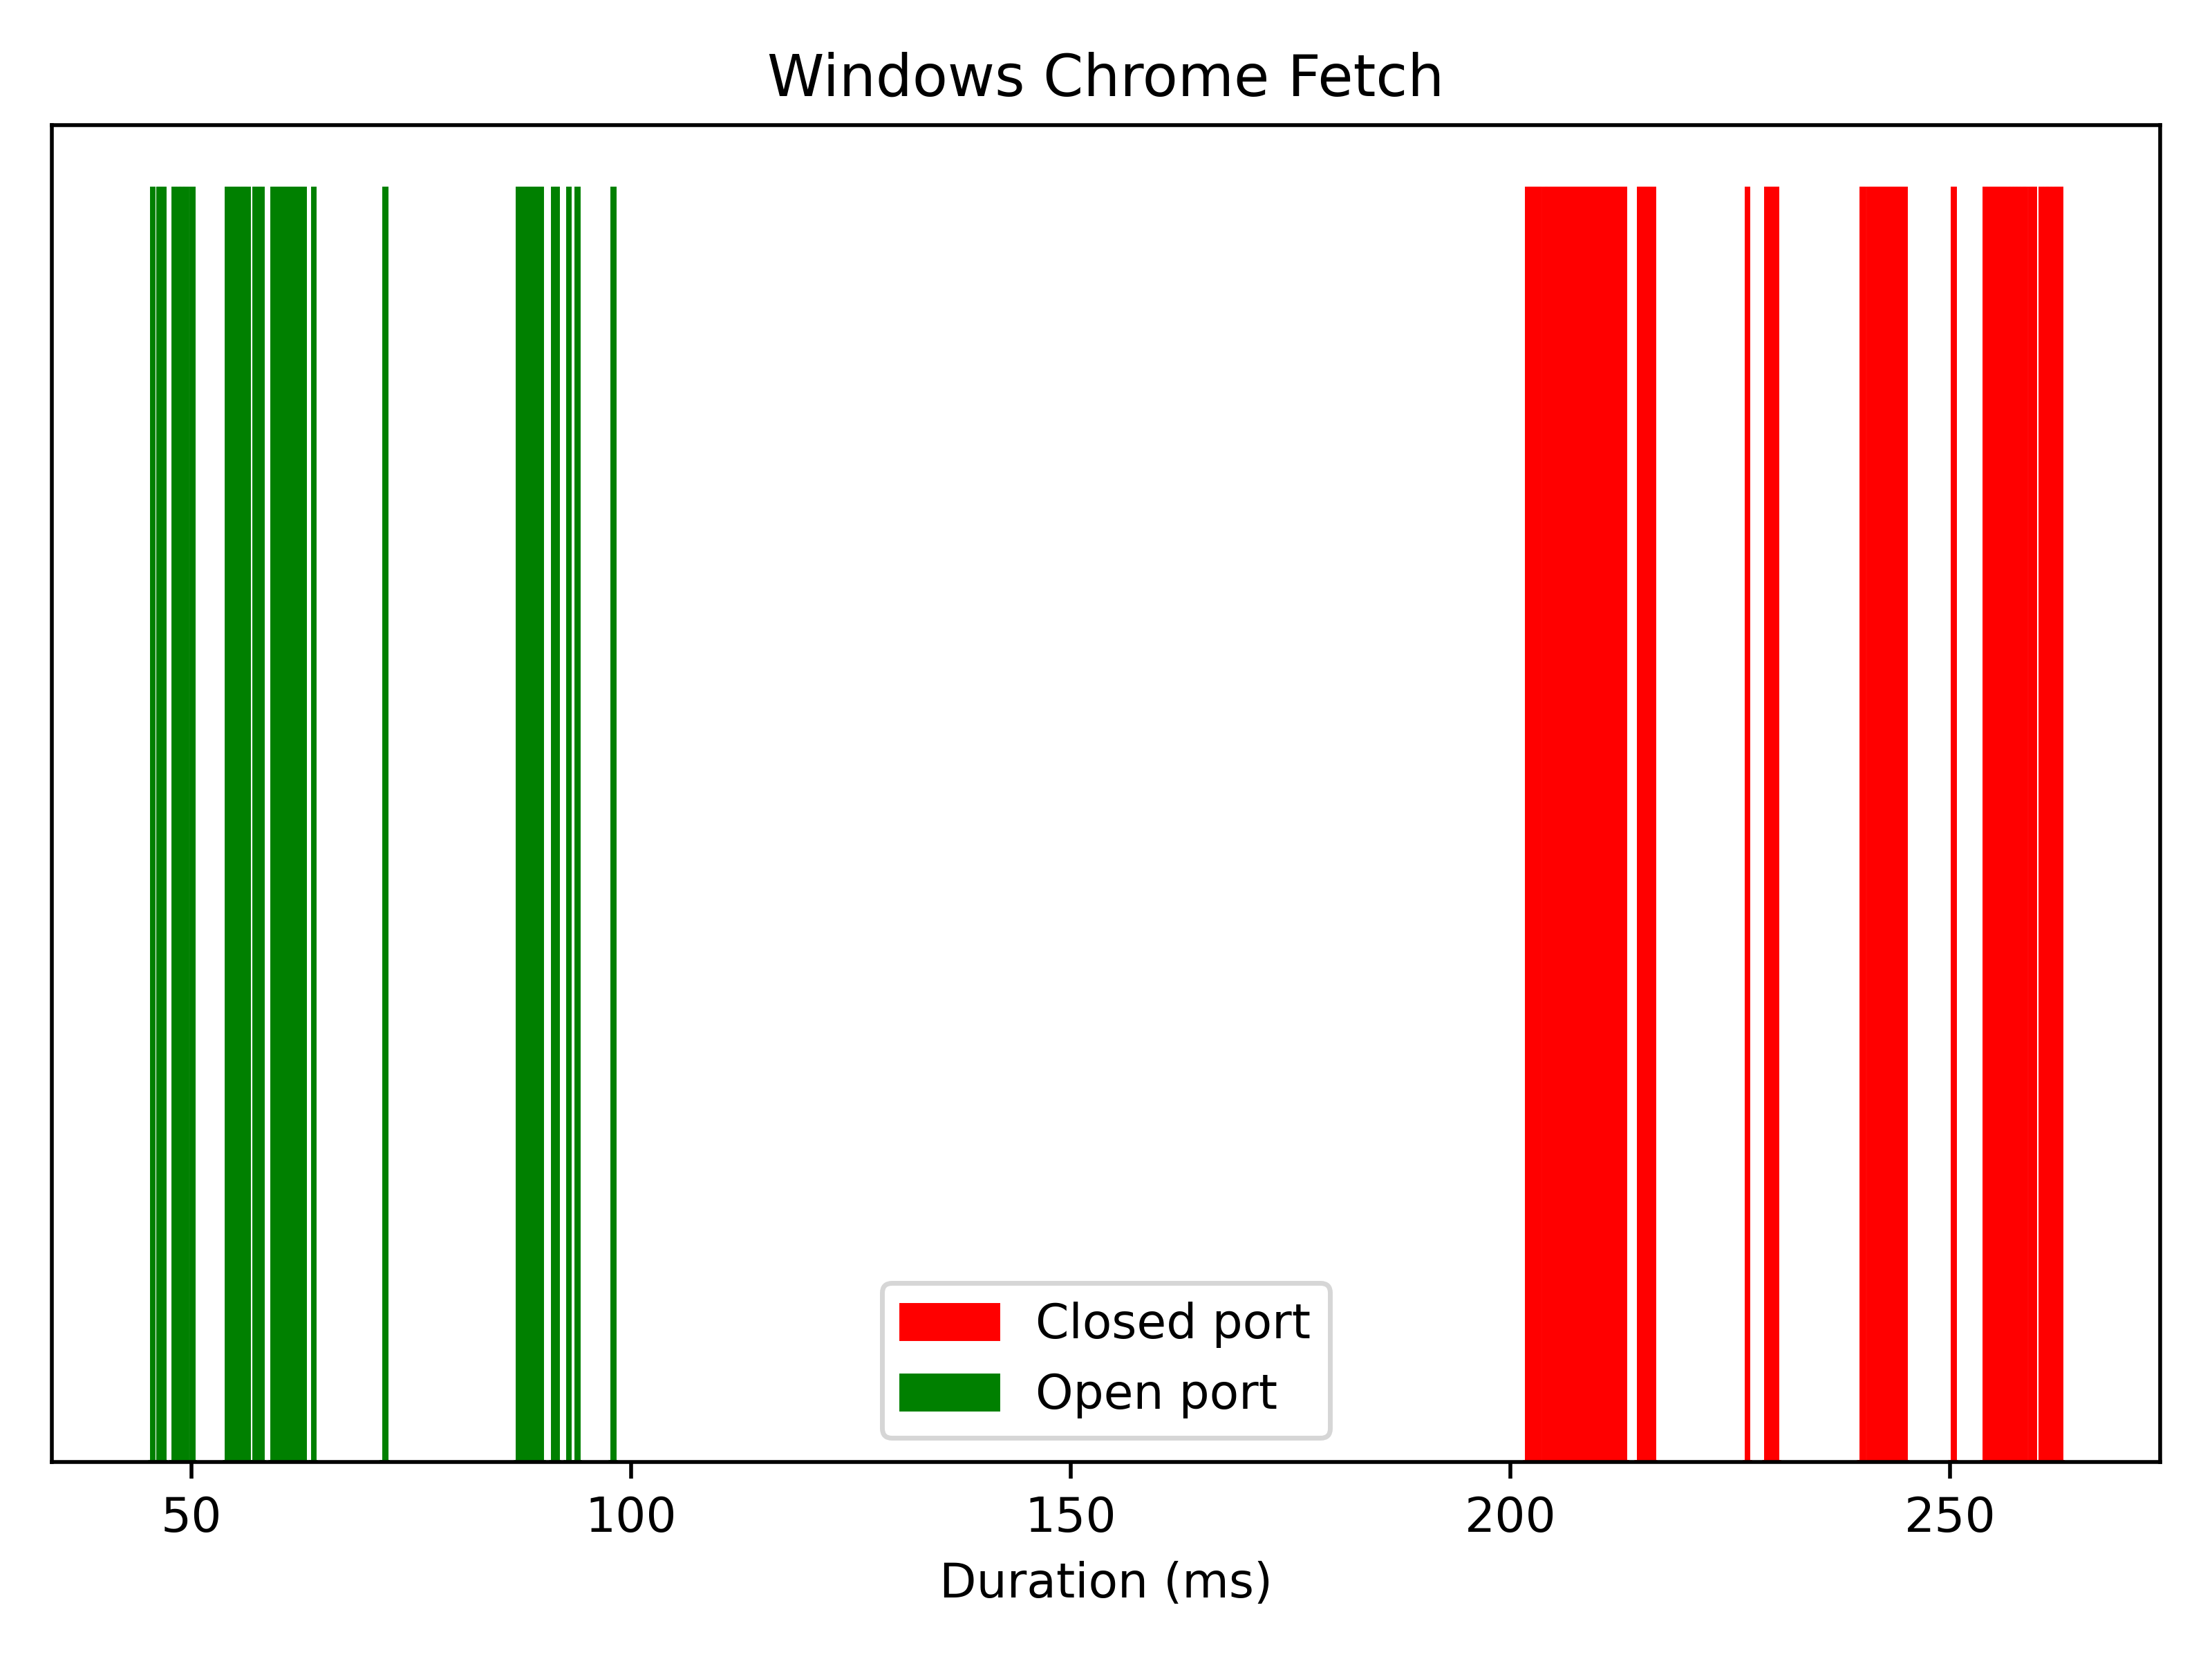
\includegraphics[width=8cm, height=4cm, keepaspectratio]{port_scanning_techniques/img/windows_chrome_efficacy_fetch.png}
    \caption{Windows/Chrome Fetch API scan duration open vs closed ports}
    \label{fig:win-chrome-fetch}
\end{minipage}
\hspace{0.5cm} % Adjust the horizontal space between the two figures
\begin{minipage}{.45\textwidth}
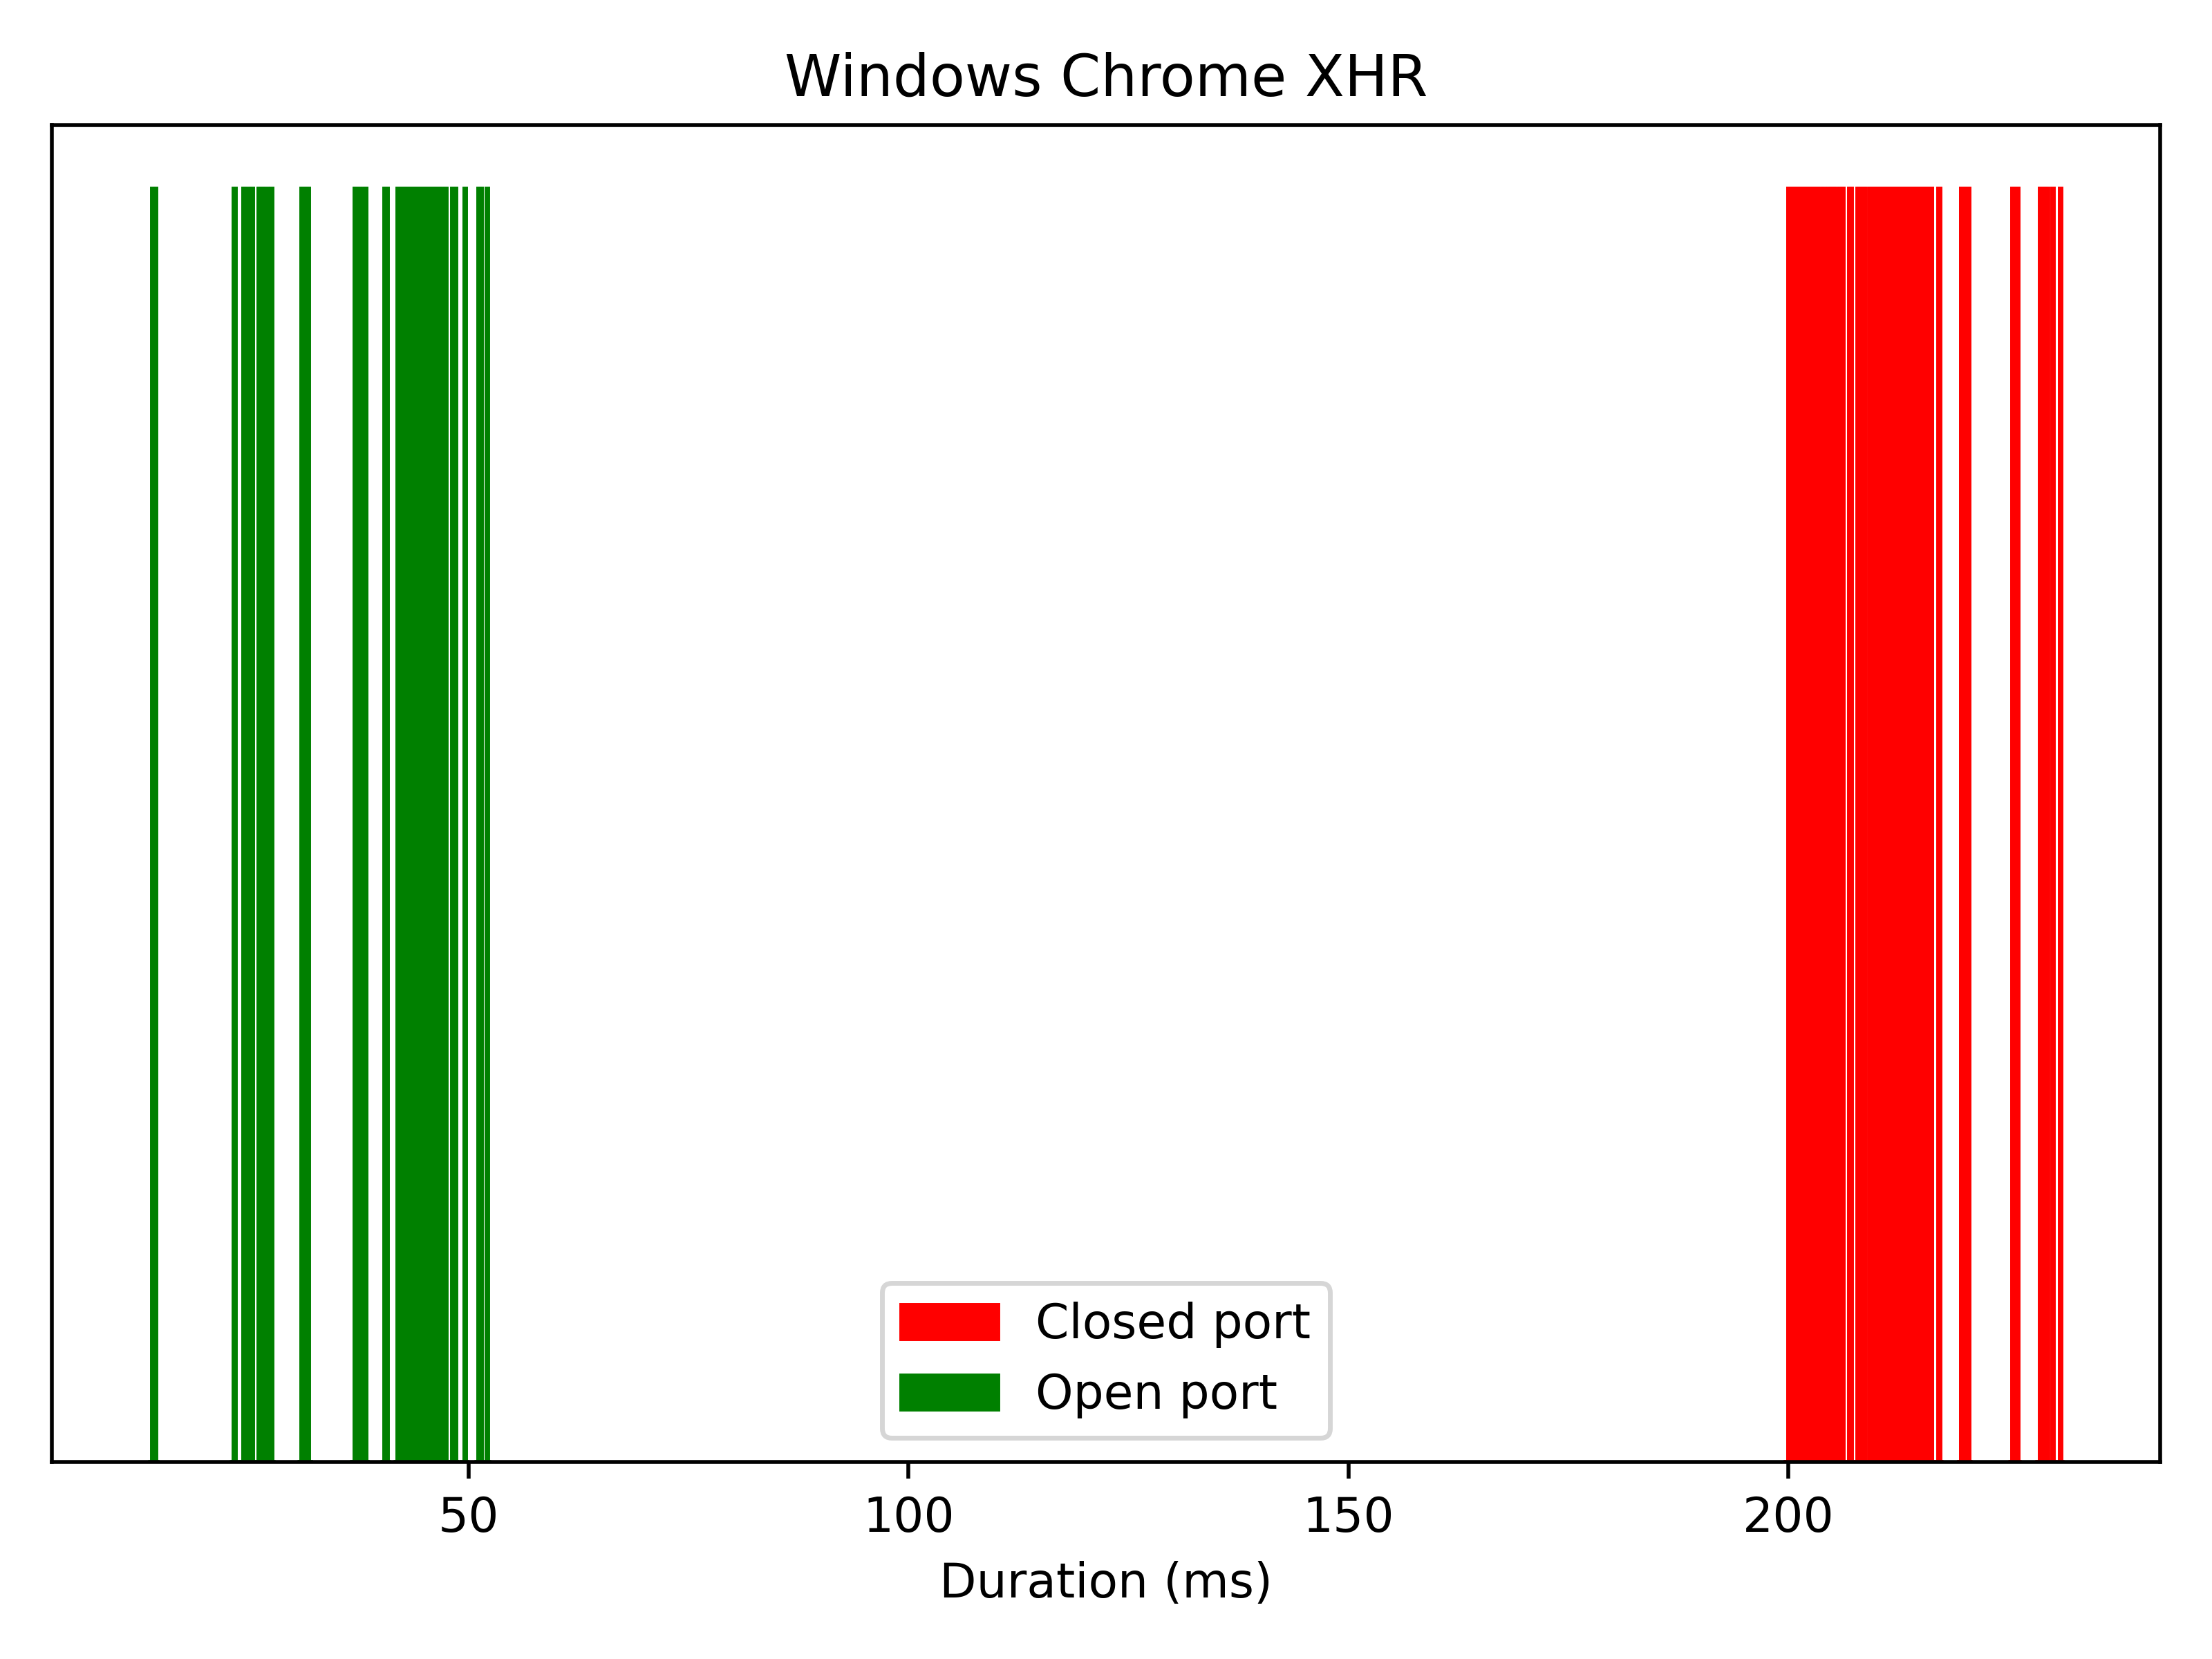
\includegraphics[width=8cm, height=4cm, keepaspectratio]{port_scanning_techniques/img/windows_chrome_efficacy_xhr.png}
    \caption{Windows/Chrome XHR API scan duration open vs closed ports}
    \label{fig:appendix-win-chrome-xhr}
\end{minipage}
\end{figure}

\begin{figure}[ht]
\centering
\begin{minipage}{.45\textwidth}
  \centering
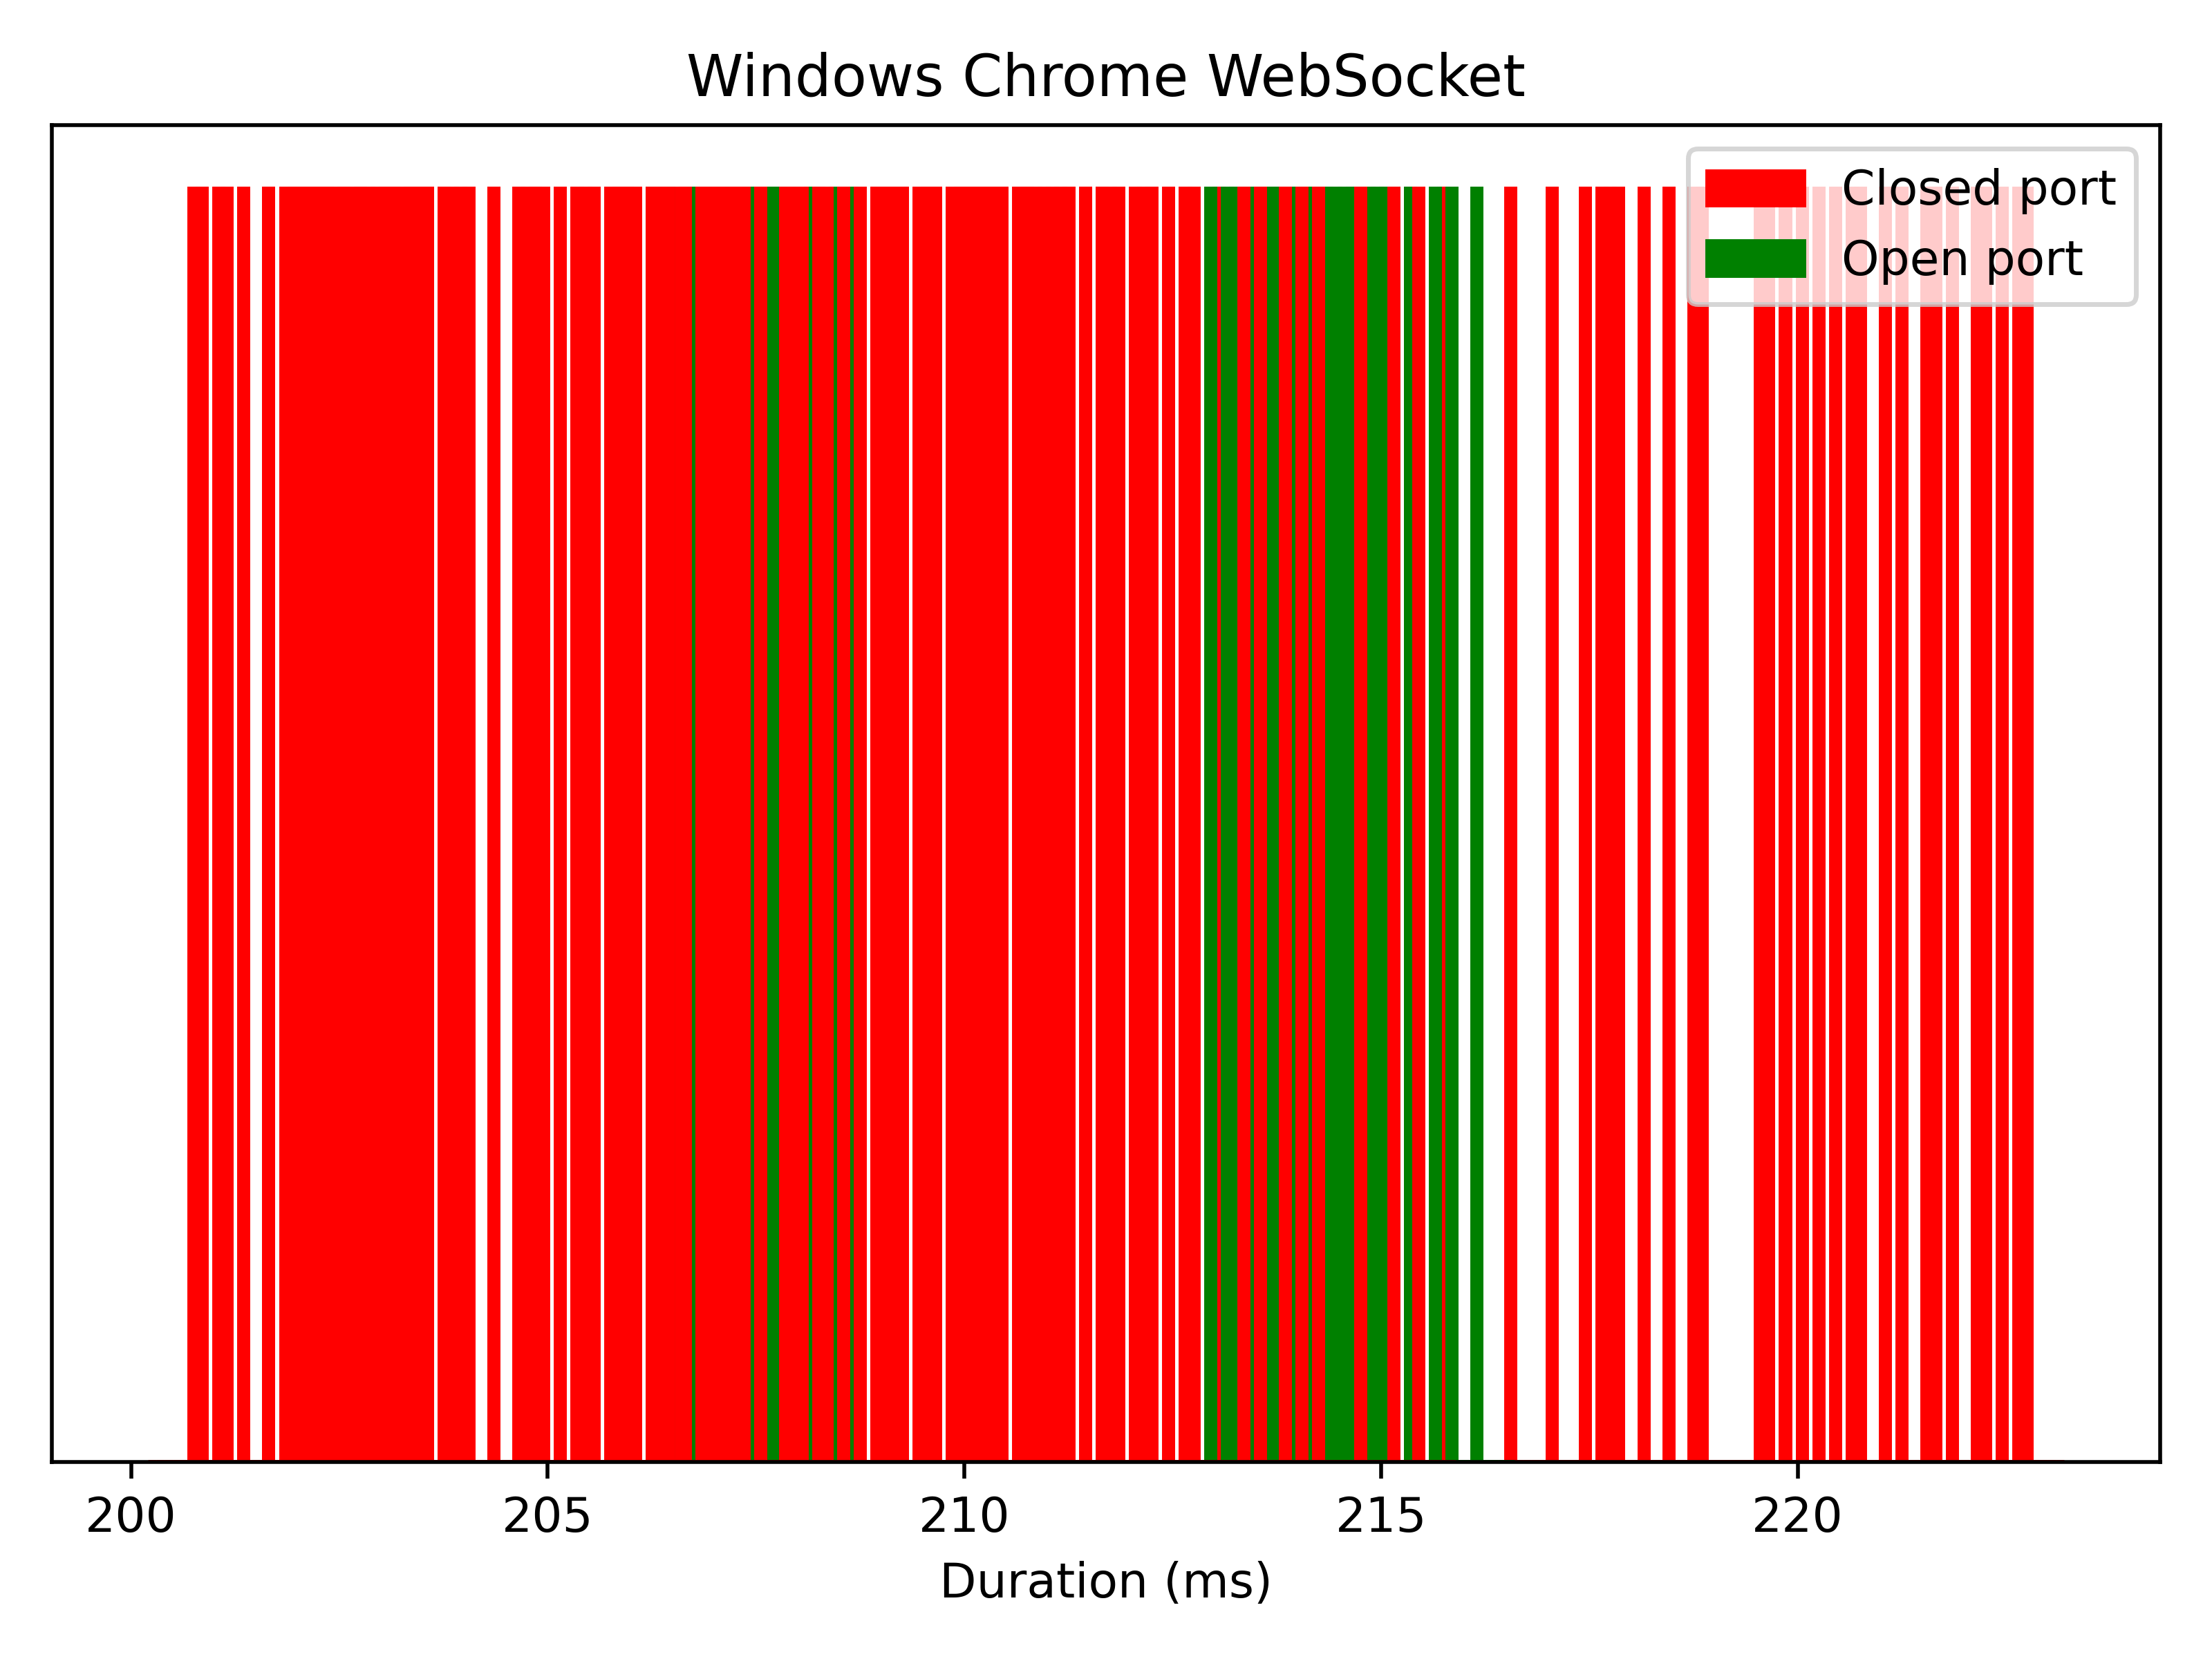
\includegraphics[width=8cm, height=4cm, keepaspectratio]{port_scanning_techniques/img/windows_chrome_efficacy_websocket.png}
    \caption{Windows/Chrome WebSocket API scan duration open vs closed ports}
    \label{fig:appendix-win-chrome-websocket}
\end{minipage}
\hspace{0.5cm} % Adjust the horizontal space between the two figures
\begin{minipage}{.45\textwidth}
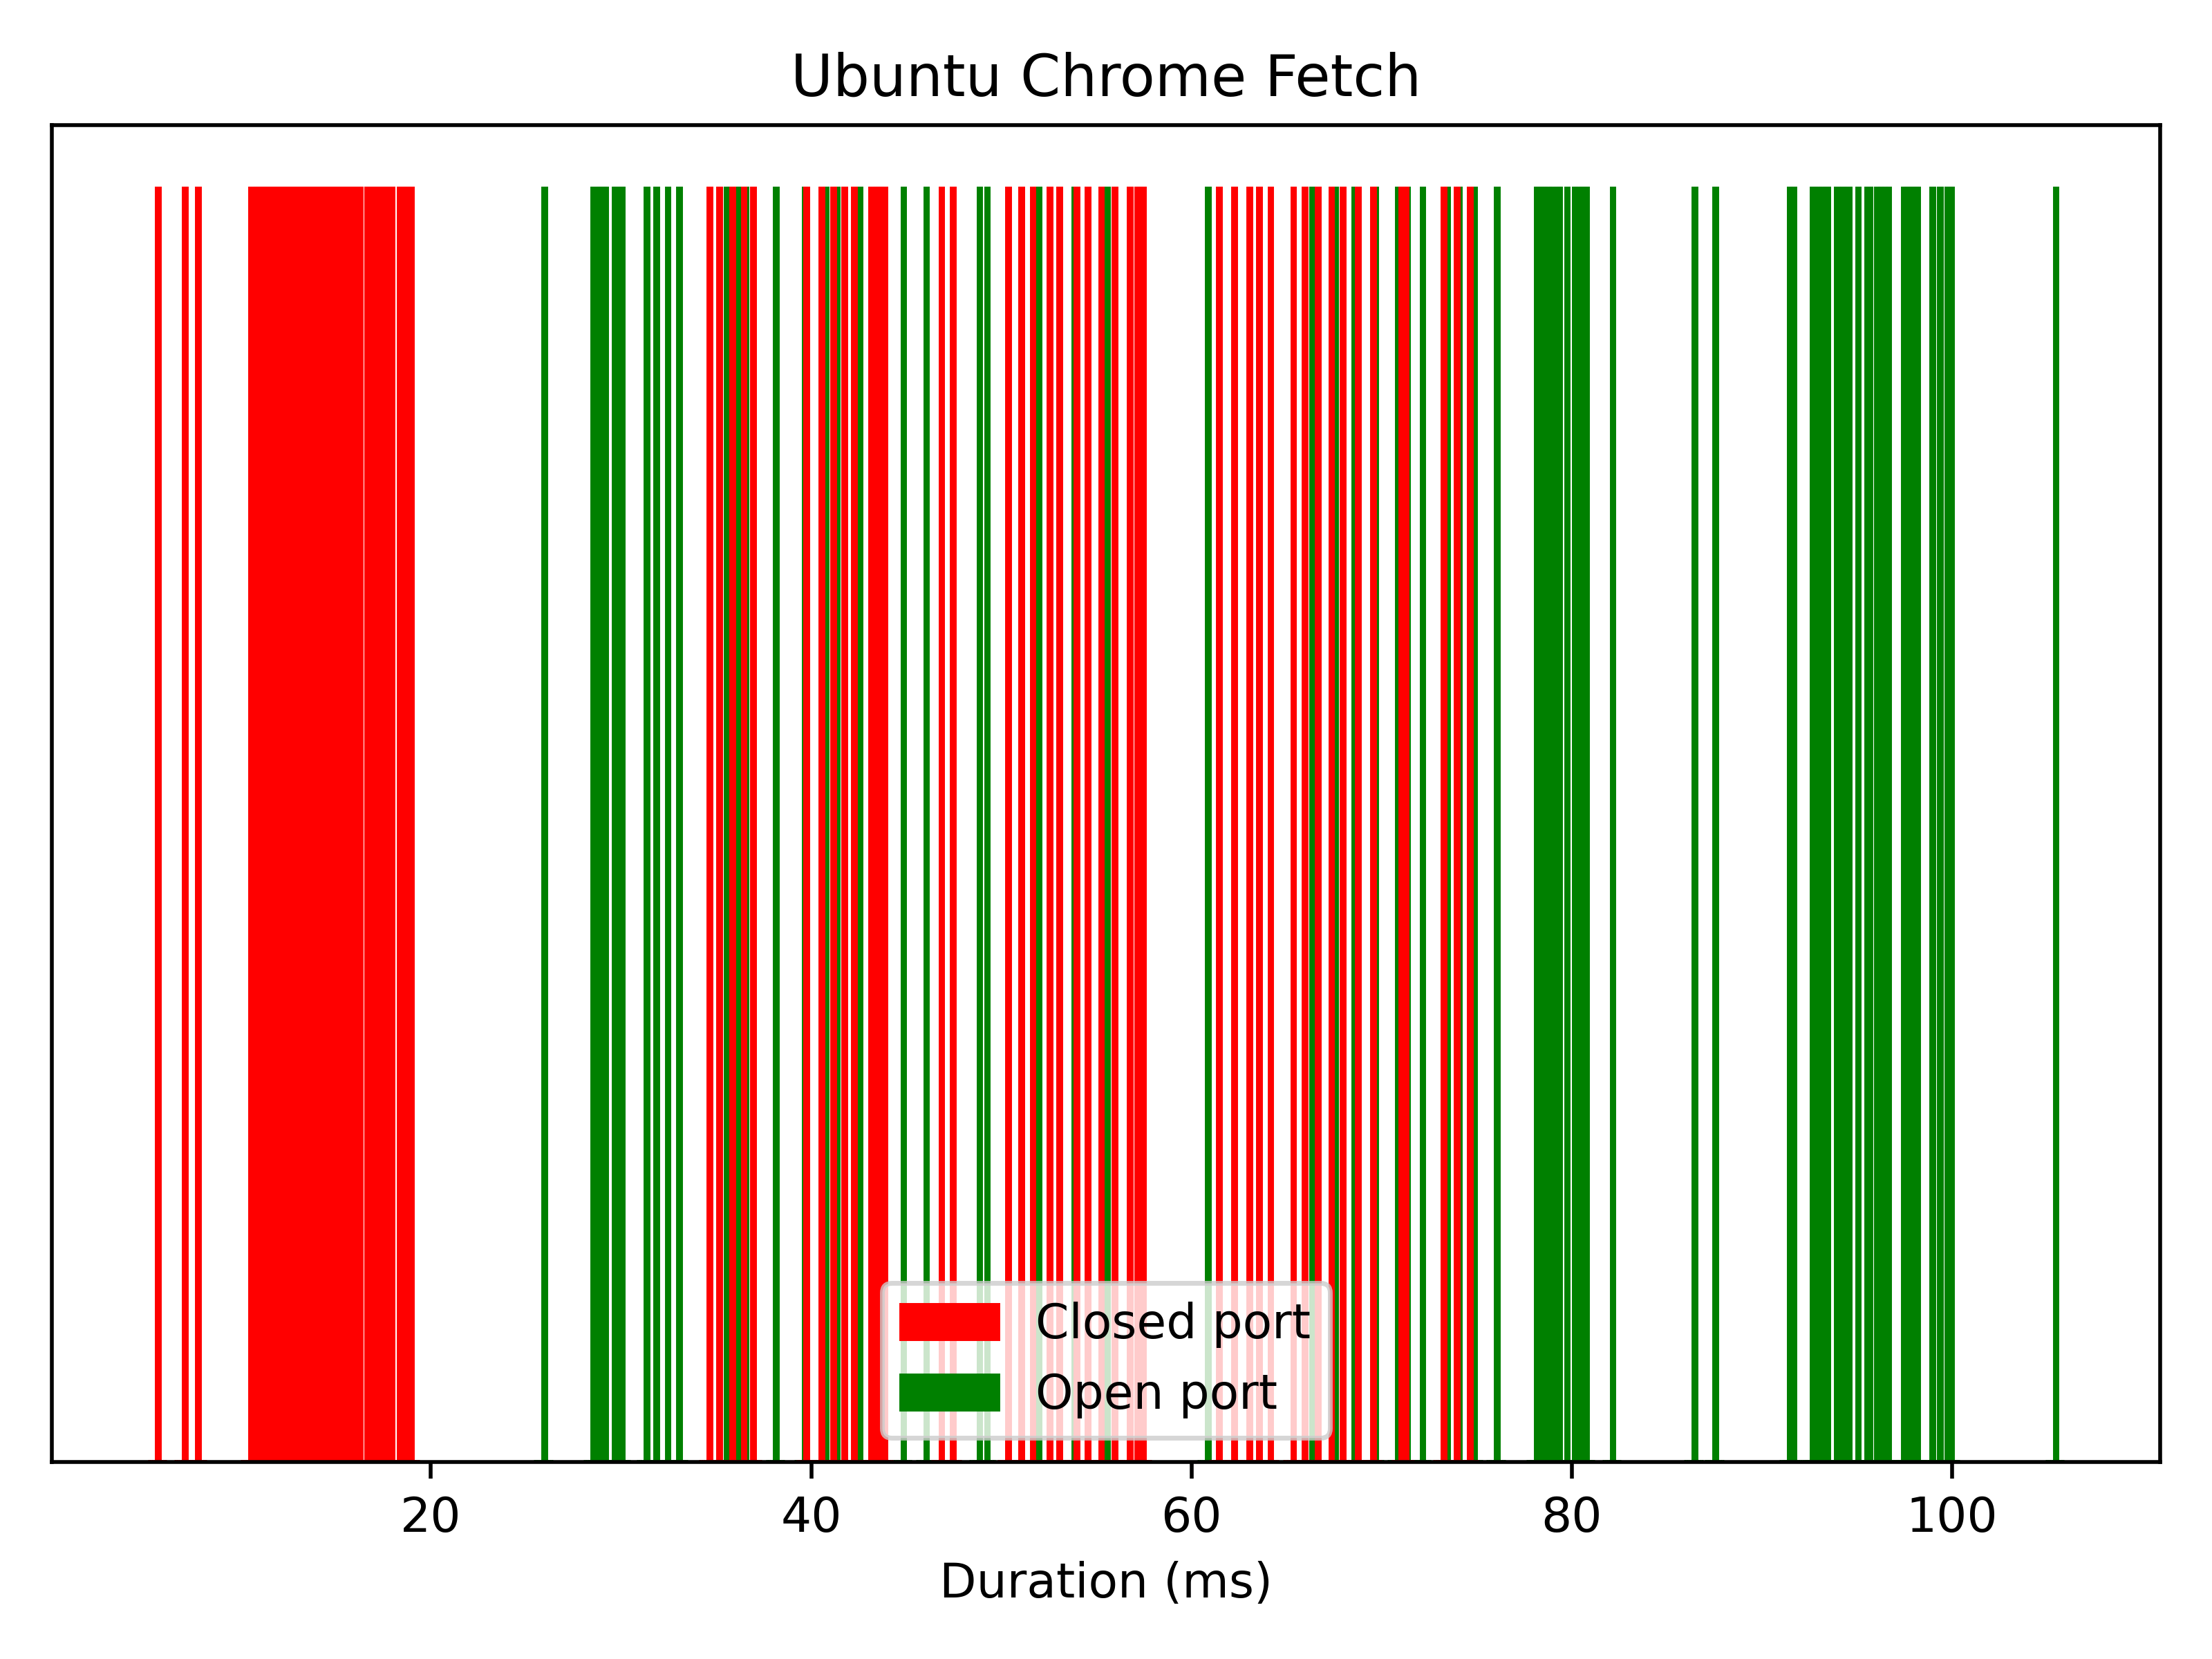
\includegraphics[width=8cm, height=4cm, keepaspectratio]{port_scanning_techniques/img/ubuntu_chrome_efficacy_fetch.png}
    \caption{Ubuntu/Chrome Fetch API scan duration open vs closed ports}
    \label{fig:ubuntu-chrome-fetch}
\end{minipage}
\end{figure}

\begin{figure}[ht]
\centering
\begin{minipage}{.45\textwidth}
  \centering
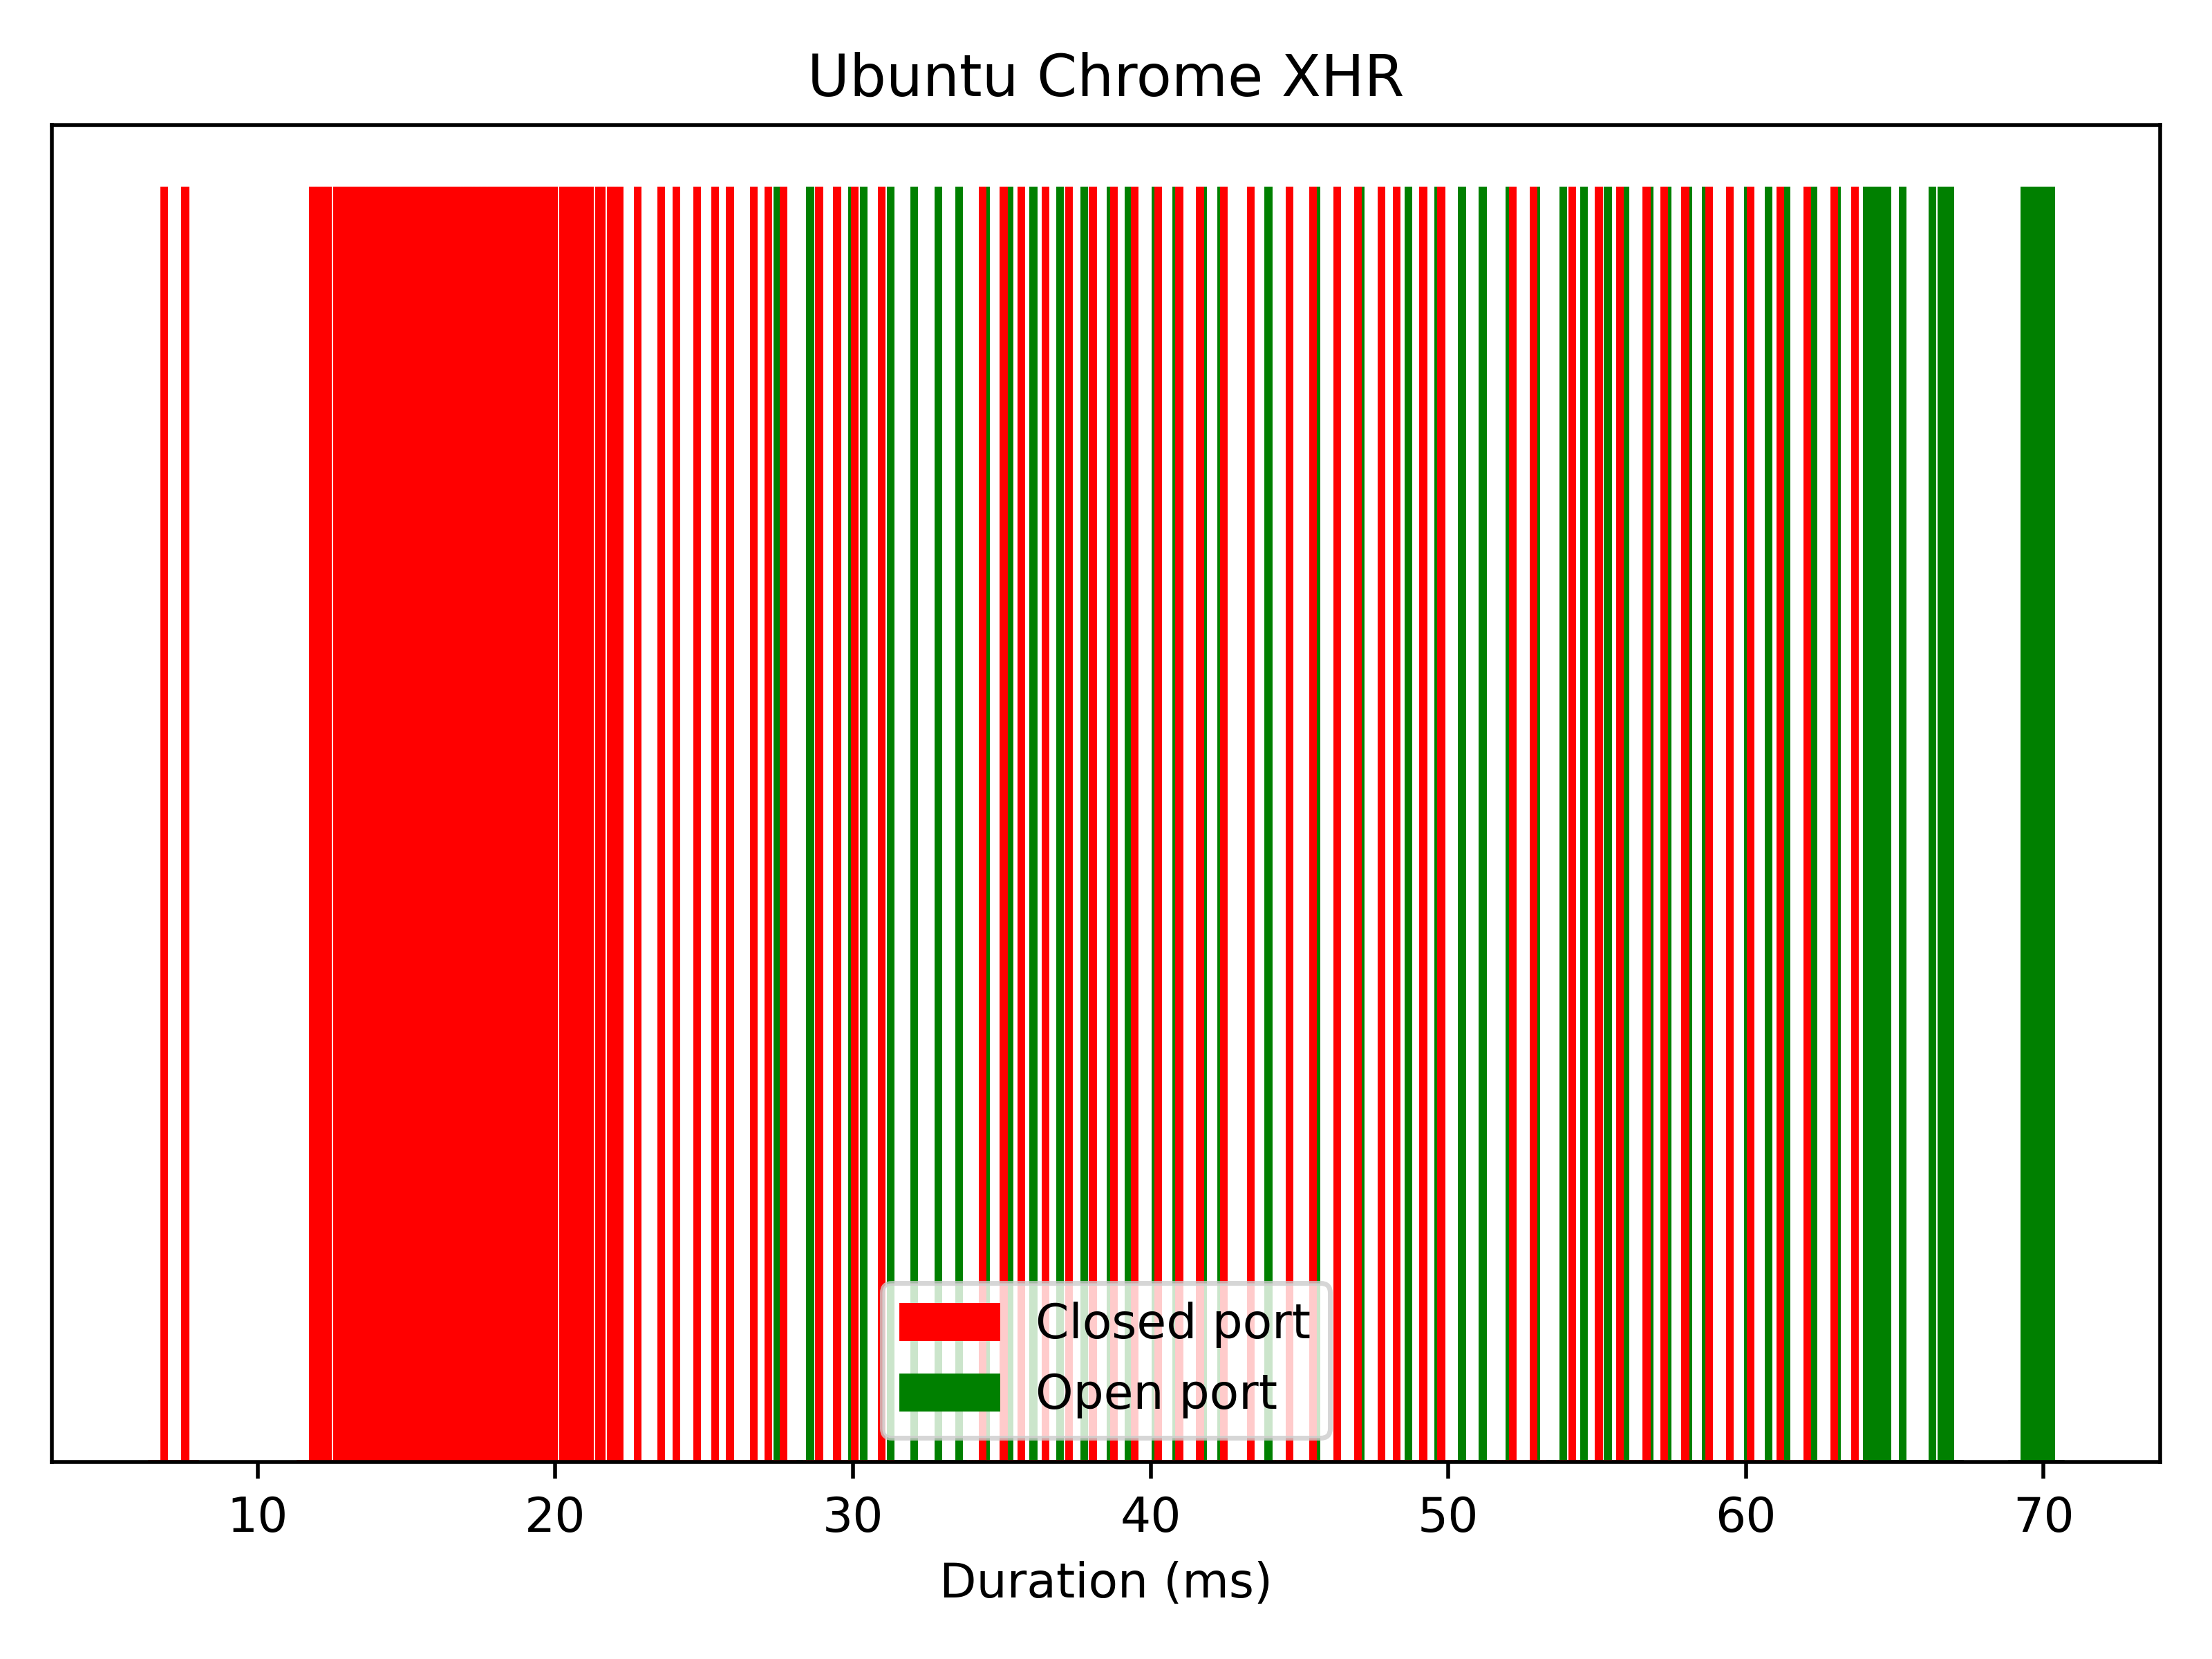
\includegraphics[width=8cm, height=4cm, keepaspectratio]{port_scanning_techniques/img/ubuntu_chrome_efficacy_xhr.png}
    \caption{Ubuntu/Chrome XHR API scan duration open vs closed ports}
    \label{fig:ubuntu-chrome-xhr}
\end{minipage}
\hspace{0.5cm} % Adjust the horizontal space between the two figures
\begin{minipage}{.45\textwidth}
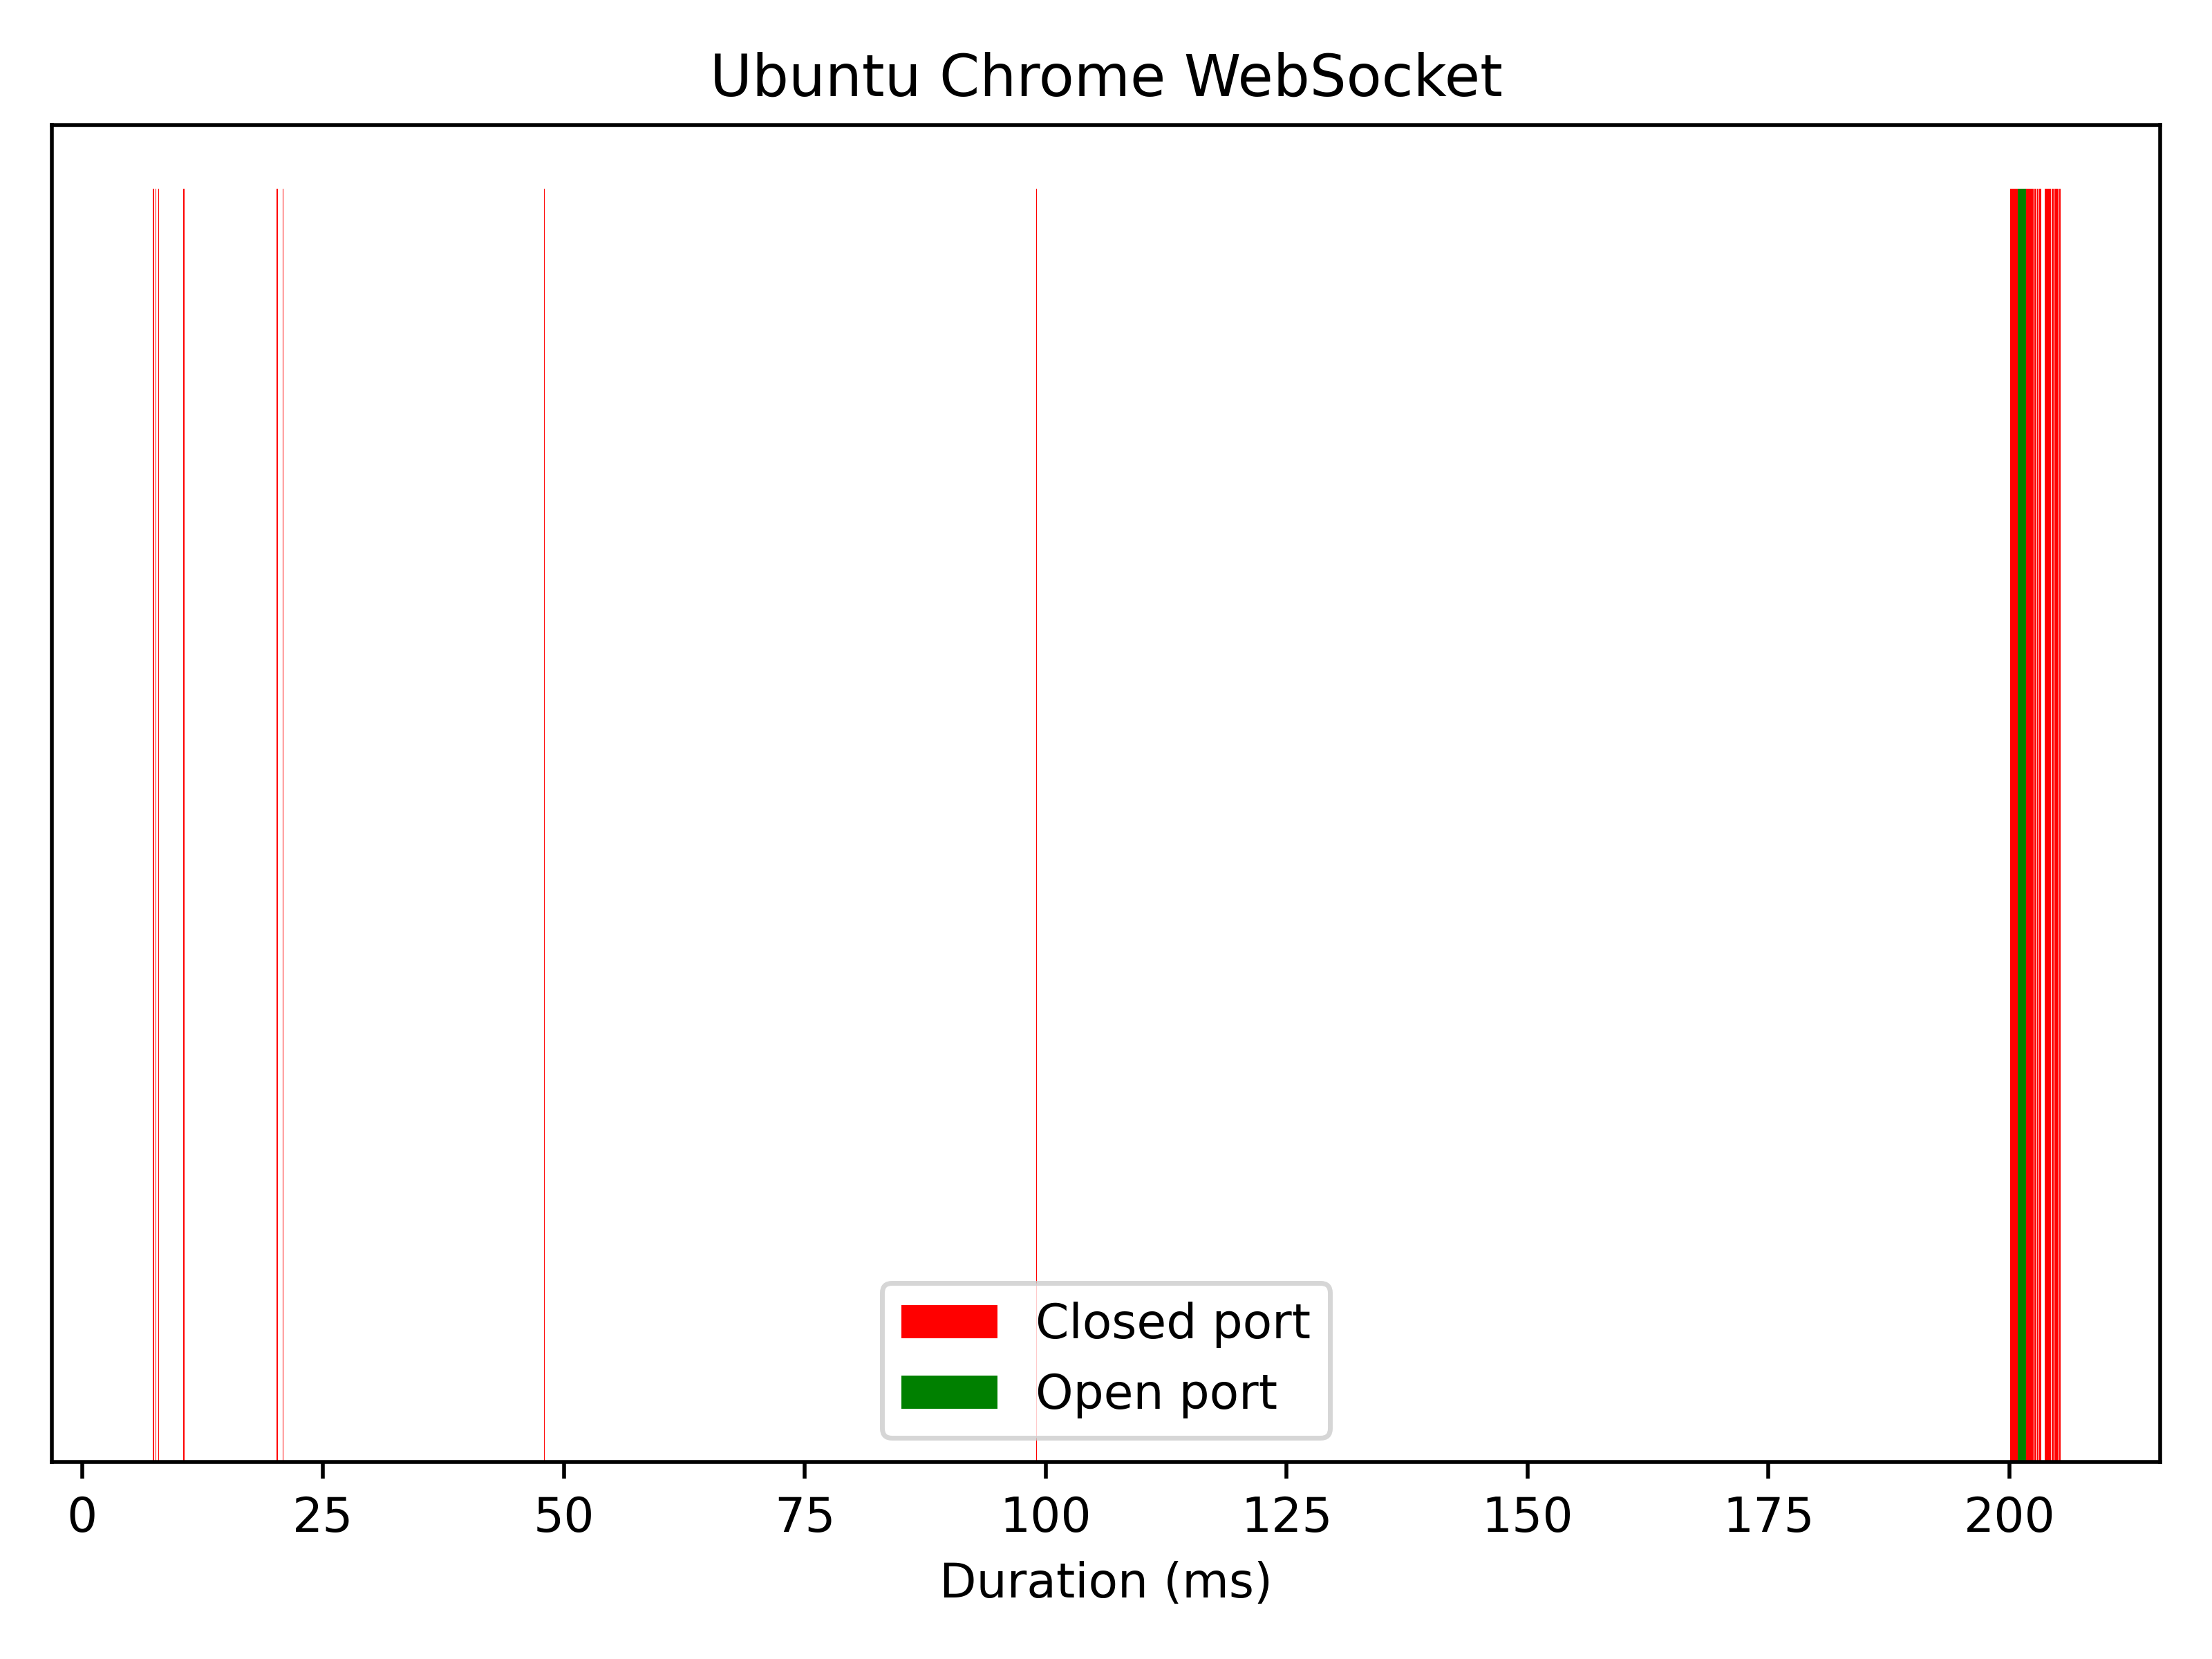
\includegraphics[width=8cm, height=4cm, keepaspectratio]{port_scanning_techniques/img/ubuntu_chrome_efficacy_websocket.png}
    \caption{Ubuntu/Chrome WebSocket API scan duration open vs closed ports}
    \label{fig:ubuntu-chrome-websocket}
\end{minipage}
\end{figure}

\begin{figure}[ht]
\centering
\begin{minipage}{.45\textwidth}
  \centering
\includegraphics[width=8cm, height=4cm, keepaspectratio]{port_scanning_techniques/img/windows_Firefox_efficacy_fetch.png}
    \caption{Windows/Firefox Fetch API scan duration open vs closed ports}
    \label{fig:win-firefox-fetch}
\end{minipage}
\hspace{0.5cm} % Adjust the horizontal space between the two figures
\begin{minipage}{.45\textwidth}
\includegraphics[width=8cm, height=4cm, keepaspectratio]{port_scanning_techniques/img/windows_Firefox_efficacy_xhr.png}
    \caption{Windows/Firefox XHR API scan duration open vs closed ports}
    \label{fig:appendix-win-firefox-xhr}
\end{minipage}
\end{figure}

\begin{figure}[ht]
\centering
\begin{minipage}{.45\textwidth}
  \centering
\includegraphics[width=8cm, height=4cm, keepaspectratio]{port_scanning_techniques/img/windows_Firefox_efficacy_websocket.png}
    \caption{Windows/Firefox WebSocket API scan duration open vs closed ports}
    \label{fig:appendix-win-firefox-websocket}
\end{minipage}
\hspace{0.5cm} % Adjust the horizontal space between the two figures
\begin{minipage}{.45\textwidth}
\includegraphics[width=8cm, height=4cm, keepaspectratio]{port_scanning_techniques/img/ubuntu_Firefox_efficacy_fetch.png}
    \caption{Ubuntu/Firefox Fetch API scan duration open vs closed ports}
    \label{fig:ubuntu-firefox-fetch}
\end{minipage}
\end{figure}

\begin{figure}[ht]
\centering
\begin{minipage}{.45\textwidth}
  \centering
\includegraphics[width=8cm, height=4cm, keepaspectratio]{port_scanning_techniques/img/ubuntu_Firefox_efficacy_xhr.png}
    \caption{Ubuntu/Firefox XHR API scan duration open vs closed ports}
    \label{fig:ubuntu-firefox-xhr}
\end{minipage}
\hspace{0.5cm} % Adjust the horizontal space between the two figures
\begin{minipage}{.45\textwidth}
\includegraphics[width=8cm, height=4cm, keepaspectratio]{port_scanning_techniques/img/ubuntu_Firefox_efficacy_websocket.png}
    \caption{Ubuntu/Firefox WebSocket API scan duration open vs closed ports}
    \label{fig:ubuntu-firefox-websocket}
\end{minipage}
\end{figure}
\clearpage

\section{Scanning techniques efficiency comparison}
\label{appendix:efficiency-comparison}

\begin{figure}[ht]
\begin{adjustwidth}{-3cm}{-1cm}
\centering
\begin{minipage}{.45\textwidth}
  \centering
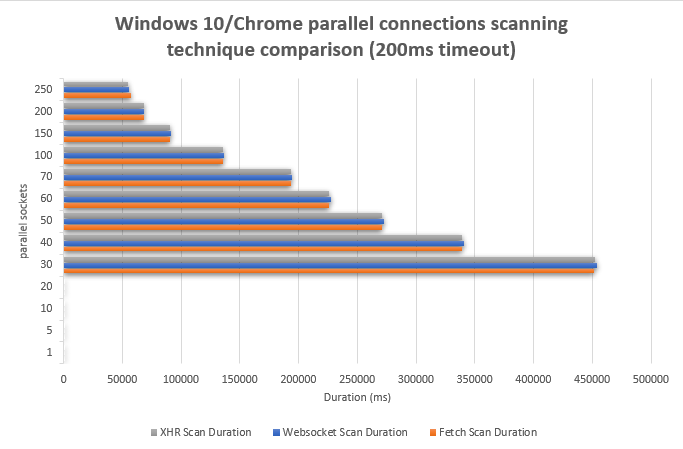
\includegraphics[width=10cm, height=7cm, keepaspectratio]{port_scanning_techniques/img/windows_chrome_scan_technique_comparison.png}
    \caption{Windows/Chrome Parallel sockets efficiency comparison}
    \label{fig:appendix-windows_chrome_n_sockets}
\end{minipage}
\hspace{3cm} % Adjust the horizontal space between the two figures
\begin{minipage}{.45\textwidth}
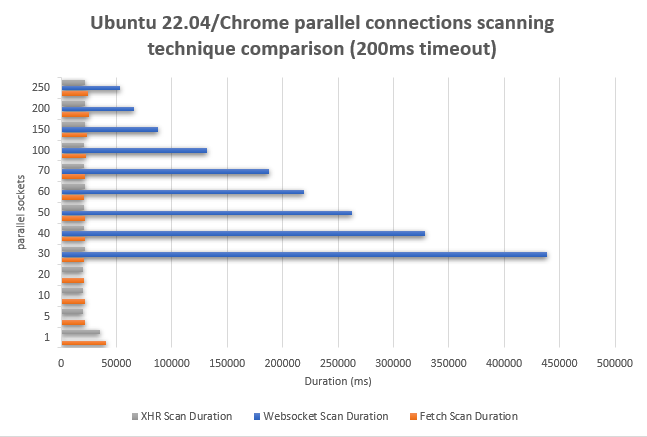
\includegraphics[width=10cm, height=7cm, keepaspectratio]{port_scanning_techniques/img/ubuntu_chrome_scan_technique_comparison.png}
    \caption{Ubuntu/Chrome Parallel sockets efficiency comparison}
    \label{fig:appendix-ubuntu_chrome_n_sockets}
\end{minipage}
\end{adjustwidth}
\end{figure}

\begin{figure}[ht]
\begin{adjustwidth}{-3cm}{-1cm}
\centering
\begin{minipage}{.45\textwidth}
  \centering
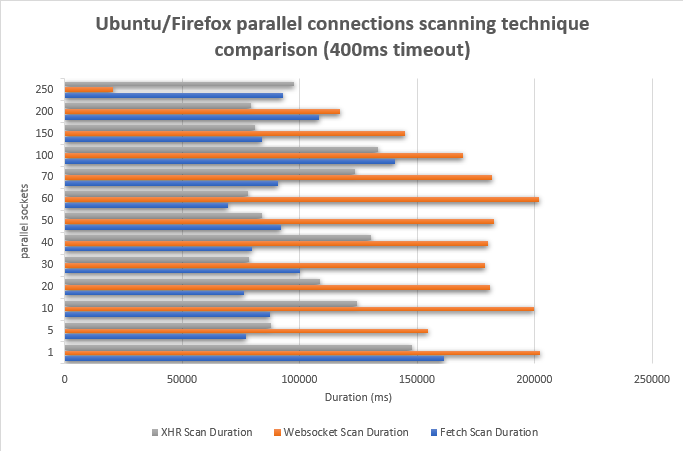
\includegraphics[width=10cm, height=7cm, keepaspectratio]{port_scanning_techniques/img/ubuntu_firefox_scan_technique_comparison.png}
    \caption{Ubuntu/Firefox Parallel sockets efficiency comparison}
    \label{fig:ubuntu_firefox_n_sockets}
\end{minipage}
\hspace{3cm} % Adjust the horizontal space between the two figures
\begin{minipage}{.45\textwidth}
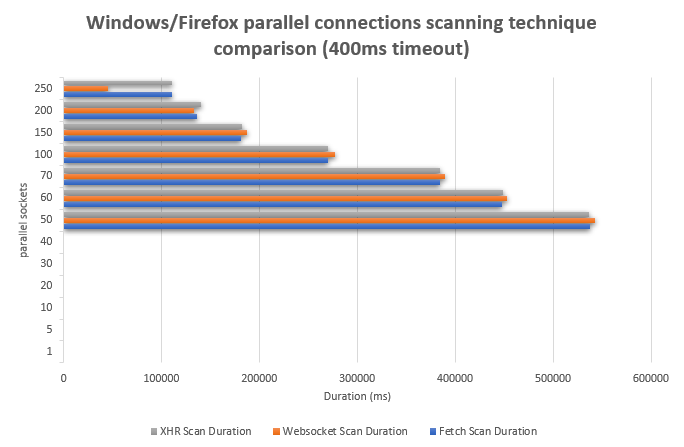
\includegraphics[width=10cm, height=7cm, keepaspectratio]{port_scanning_techniques/img/windows_firefox_scan_technique_comparison.png}
    \caption{Windows/Firefox Parallel sockets efficiency comparison}
    \label{fig:windows_firefox_n_sockets}
\end{minipage}
\end{adjustwidth}
\end{figure}
%  \input{Appendices/appendix-b}
%  \input{Appendices/appendix-c}


\end{document}
